\documentclass[journal]{IEEEtran} % or [conference] if you target a conference

% ============================================================================
% CORE PACKAGES (IEEE-style)
% ============================================================================


\usepackage{float}
\usepackage{pgfplots}
\pgfplotsset{compat=1.17}
\usetikzlibrary{shapes, arrows, positioning, calc, shapes.geometric, arrows.meta, fit, backgrounds, decorations.pathreplacing, bending}


% Recommended by IEEEtran docs for citations
% \usepackage{cite} % compressed, sorted numeric refs [web:2][web:8]
\usepackage{tabularx}
% \usepackage{natbib}
\usepackage[square,numbers,sort&compress]{natbib}
% Graphics and Figures
\usepackage{graphicx}
\usepackage{tikz}
\usetikzlibrary{shapes.geometric, arrows.meta, positioning, fit, backgrounds, calc, decorations.pathreplacing, bending}
\tikzset{>={Stealth}}

% Tables
\usepackage{booktabs}    % \toprule, \midrule, \bottomrule
\usepackage{multirow}
\usepackage{multicol}

% Mathematics
\usepackage{amsmath}
\usepackage{amssymb}
\usepackage{bm}
\usepackage{balance}
% Algorithms and Pseudocode
\usepackage{algorithm}
\usepackage{algorithmicx}
\usepackage{algpseudocode}
\usepackage{algcompatible}
% \usepackage{algorithmic} % IEEEtran-friendly (instead of algpseudocode)

% Colors and Highlighting
\usepackage{xcolor}
\usepackage{soul}        % \hl{}
\usepackage{tcolorbox}   % colored boxes for findings


% Lists and Enumeration
\usepackage{enumitem}
\setlist{nosep}

% Hyperlinks and Clever References
\usepackage[hidelinks]{hyperref}
\usepackage[nameinlink]{cleveref}

% Miscellaneous
\usepackage{url}
\usepackage{xspace}
\usepackage{comment}
\DeclareUnicodeCharacter{1D66}{\ensuremath{\beta}}

% (Optional) Units and Numbers – if you actually use siunitx
\usepackage{siunitx}
\sisetup{
  output-exponent-marker=\ensuremath{\mathrm{e}},
  group-separator={,},
  detect-weight=true,
  % detect-inline-weight=math
}

% ============================================================================
% COLOR DEFINITIONS
% ============================================================================

\definecolor{networkblue}{RGB}{52,152,219}
\definecolor{envgreen}{RGB}{46,204,113}
\definecolor{algorange}{RGB}{230,126,34}
\definecolor{allocpurple}{RGB}{155,89,182}

\definecolor{findingBlue}{RGB}{230,240,255}
\definecolor{findingRed}{RGB}{255,230,230}
\definecolor{findingOrange}{RGB}{255,245,230}
\definecolor{findingGreen}{RGB}{230,255,240}

% ============================================================================
% CUSTOM COMMANDS
% ============================================================================
% \algnewcommand\algorithmicrequire{\textbf{Input:}}
\algnewcommand\Require{\item[\algorithmicrequire]}

\newcommand{\ie}{\emph{i.e.,}\xspace}
\newcommand{\eg}{\emph{e.g.,}\xspace}
\newcommand{\etc}{etc.\xspace}
\newcommand{\etal}{\emph{et~al.}\xspace}

\newcommand{\descStep}[2]{\noindent\textbf{#1:} #2}
\newcommand{\smallTitle}[1]{\vspace{1mm}\noindent\textit{#1:}}
\newcommand{\fillin}[1]{\textcolor{gray}{\emph{[#1]}}}
\newcommand{\metric}[1]{\textsc{#1}}

\newcommand{\pp}{\,\%}
\newcommand{\SEM}{\text{SEM}}
\newcommand{\eff}{\text{Eff}}
\newcommand{\retries}{\text{Retries}}
\newcommand{\uthresh}{\text{UnderThresh}}
\newcommand{\varseed}{\text{Var}_{\text{seeds}}}

\newcommand{\Fb}{F_{\text{b}}}
\newcommand{\Tb}{T_{\text{b}}}
\newcommand{\TwoT}{2T}

% Author comments (remove for camera-ready)
\newcommand{\todo}[1]{\textcolor{cyan}{\textbf{[TODO: #1]}}}
\newcommand{\dan}[1]{\textcolor{blue}{\textit{[Dan: #1]}}}
\newcommand{\piter}[1]{\textcolor{green}{\textit{[Piter: #1]}}}

% ============================================================================
% CLEVEREF CUSTOMIZATION
% ============================================================================

\crefname{section}{Section}{Sections}
\Crefname{section}{Section}{Sections}
\crefname{figure}{Figure}{Figures}
\Crefname{figure}{Figure}{Figures}
\crefname{table}{Table}{Tables}
\Crefname{table}{Table}{Tables}
\crefname{equation}{Equation}{Equations}
\Crefname{equation}{Equation}{Equations}
\crefname{algorithm}{Algorithm}{Algorithms}
\Crefname{algorithm}{Algorithm}{Algorithms}

% ============================================================================
% TYPOGRAPHY / SPACING TWEAKS (light-touch for IEEE)
% ============================================================================

% Avoid widows/orphans
\widowpenalty=10000
\clubpenalty=10000

% Slightly tighter lists
\setlist[itemize]{topsep=2pt, partopsep=0pt, itemsep=2pt, parsep=0pt}
\setlist[enumerate]{topsep=2pt, partopsep=0pt, itemsep=2pt, parsep=0pt}

\begin{document}

\title{XXXXX}

\author{First Author,~Second Author,~and~Third Author%
\thanks{Affiliations and funding info here.}}

\maketitle





% % [Provide some background similar to Jie's work here]

% % Most existing research assumes that the success rates of entanglement links between neighboring quantum nodes are already known. This is problematic because real-world quantum networks exhibit highly dynamic, time-varying link fidelities that cannot be reliably estimated in advance, making fixed or assumed success rates unrealistic and leading to suboptimal or brittle routing and allocation decisions. In contrast, this paper tackles the online problem of determining the optimal path and qubit allocation strategy — aiming to learn, in real time, how to maximize the success rate of entanglement between two chosen quantum computers without prior knowledge of link performance. \hl{The proposed method employs a multi-armed bandit (MAB) framework, specifically `informed Contextual Multi-Armed Bandits' (iCMAB) approach, which models each potential path as a group and treats qubit allocation decisions as arm selections.}
% \dan{Piter: Update with how our model works} Our contributions include: I) % 2-4 high level impacts of our work


% % Should we also mention if the source code is available on the project website


% %%%%%%%%%%%%%%%%%%%%%%%%%%%%%%%%%%%%%%%%%%%%%%%%%%%%%%%%
% % DK: Perhaps bounce the idea of of Stefan
% %   DK: Consider doing the experiment using their QDN if applicable. Do it in a paper or even a grant. See how we can piggy back on their effort.
% % 
% %

% ---


% DK: Other things to look at:


% wang2025learning
% - Path vs link level? Does Jie do this and does it make sense to do this?
% - Are we doing quantum data networks or quantum networks
% - What else can be borrowed/contrasted from this paper?
% - Does it make sense to compare our work against this process? 
% ? How do we deal with the path explosion problem?
% ? Are we dealing with a one way or two way quantum network



% ? Herealded entanglement generation
% One way, two way quantum network


% Pauli
% Clifford operation



\begin{abstract}

\dan{Piter: Did you speak with Travis regarding this yet?}




\todo{Dan: Take a shot at the abstract and intro}


- Be sure to compare against \cite{10621263}

% Most existing quantum routing research assumes that entanglement success rates between nodes are known or can be accurately estimated. This assumption is unrealistic: real-world quantum networks exhibit dynamically varying link fidelities due to decoherence, hardware fluctuations, and adversarial interference—characteristics that defy static estimation and render fixed-rate designs brittle.

% We address the online learning problem of jointly optimizing entanglement path selection and qubit allocation in real time without prior link-performance knowledge. Through systematic evaluation across 370+ experimental conditions spanning 13 algorithms, 5 scenarios (Stochastic, Markov, Adaptive, OnlineAdaptive, Baseline), 4 allocator strategies, and 2 capacity settings at mid-range horizons (4K--8K frames), we uncover fundamental insights into routing robustness under compound uncertainty.


% \dan{We can talk about this, but maybe something where we discuss it being a problem. Maybe something like: We demonstrate that XYZ is a problem... Just a thought.}
% The problem that we are solving is that ?assuming that entanglement success rates are static leads to lower fidelity? <-- It would be good if we can cite this someplace

Quantum entanglement routing requires dynamic path selection and qubit allocation under noisy, uncertain, and adversarial conditions. Existing routing approaches often assume stationary link behavior, decouple selection from allocation, or rely on offline optimization—assumptions that break when link fidelities drift and disruptions adapt to the learner.

We present a systematic evaluation of context-aware pursuit neural bandit algorithms for joint path selection and qubit allocation in quantum networks\dan{Is tehre just an evaluation that is done, or is there something new proposed? If someething new is proposed, it should be mentioned here}. Across 552 configurations spanning 13 algorithms, 5 threat scenarios (Stochastic, Markov, Adaptive, OnlineAdaptive, Baseline), 4 allocator strategies, and 2 capacity settings, pursuit--neural hybrids (\texttt{CPursuitNeuralUCB}, \texttt{iCPursuitNeuralUCB}) emerge as the most robust family, achieving 86--89\% oracle-normalized efficiency on average and approaching 90\% under favorable capacity--allocator regimes. They outperform non-contextual bandit baselines by 18--24 percentage points (pp) and sustain higher worst-case performance under strategic attacks than adversarial-first designs.

Most critically, we uncover a \emph{capacity paradox}: increasing replay capacity from $T$ to $2T$ can induce a 22--31 pp efficiency collapse under Adaptive attacks, indicating that resource \emph{predictability}, not bandwidth, limits robustness against intelligent adversaries. Allocator choice further induces 10--15 pp swings for identical algorithms, establishing algorithm--allocator co-design as a deployment requirement. We derive threat-responsive allocation guidelines that yield 86--90\% efficiency versus 68--77\% for non-contextual baselines, suggesting broader applicability to resource-constrained online decision systems facing intelligent adversaries.

\end{abstract}



\maketitle


% \dan{dan}\piter{piter}\todo{todo}\hl{hi}
% %%%%%%%%%%%%%%%%%%%%%%%%%%%%%%%%%%%%%%%%%%%%%%%%%%%%%%%%%

% \dan{Piter: Do we want to do anything with qubit allocation? Are we doing anything with qubit allocation?}




% %%%%%%%%%%%
% %% <Figure out which areas we are examining and then look at how we are including them in the paper>

% % Introduction to things
% % What is the problem
% % What our solution is
% % What are our results

% Quantum data networks (QDNs)

% - Jie's paper incorporates neural network-based contextual information to predict outcomes for paths that haven’t been fully tried yet, making the exploration smarter than pure random selection. How do we compare against this?





% To summarize, this work makes the following contributions:


% \begin{itemize}[leftmargin=2em]%[leftmargin=*]

%     \item \descStep{Problem Demonstration}{We ?further? demonstrate the adverse impact of stochastic scenarios on Entanglement path selection and Qubit allocation \dan{Piter: Are there any papers that already demonstrate the adverse impact of stochastic-ness on entanglement path selection}} % DK: Also, are we doing just path selection or also qubit allocation?.}
%     \item \descStep{Demonstration of Capabilities}{We demonstrate the proficiency of our XYZ technique in relation to the state of the art for both stochastic and adversarial scenarios for path selection.}
%     \item \descStep{Simulation and Dataset Availability}{XXXXX.} % DK: Obviously only state this if we do it.

% ---
    
% %    \item \descStep{Robust Simulations}{We conduct robust simulation to demonstrate the benefits of our proposed XYZ process over existing bandit algorithms.}
% %    \item \descStep{XXXX}{XXXXX.}
% %    \item \descStep{XXXX}{XXXXX.}

% \end{itemize}

% %The rest of the paper is organized as follows: Section~\ref{sec: developedLab} presents our created experiential education lab, and Section~\ref{sec: studydesign} discusses the design of our study. Evaluation results are provided in Section~\ref{sec: Evaluation} and Section~\ref{sec: Discussion} discusses the findings of our research. Section~\ref{sec: RelatedWork} presents related works, and Section~\ref{sec: Conclusion} provides a conclusion.
% %\dan{update everything above}

\section{Introduction}
\todo{I need to clean this part up}
%   DK: The general writing needs to be made more clear

% Background
% WHat is the problem that we are solving/why should people care
% How did we solve it
% What were our findings.




\dan{somepleace likely add in a paragraph that describes why quantum networking path determination is `unique' to traditional routing or even path determination} % DK: Perhaps do a paragraph for this
% %%% Some examples
%   Entanglement distribution instead of data packets
%   No copying or amplification
%   Fidelity degradation
%   Probabilistic success rates

%       DK: Be sure to use some citations for these


\dan{Would it make sense to include a flowchart early on?}

Quantum entanglement distribution is a foundational primitive of the quantum Internet, enabling applications ranging from quantum key distribution (QKD) to distributed quantum computing~\cite{kimble2008quantum,wehner2018quantum,wootters1982single,bennett1993teleporting}. Yet reliable end-to-end entanglement is difficult to sustain: quantum states are fragile, entanglement generation and swapping are probabilistic, and performance degrades rapidly under decoherence and interference. In repeater-based architectures~\cite{briegel1998quantum}, entanglement swapping introduces stochastic waiting-time effects that compound along multi-hop routes~\cite{wang2019waiting}. These properties create a sequential decision problem in which a routing agent must repeatedly select among candidate paths while learning from noisy outcomes, making multi-armed bandits (MABs) a natural abstraction for online path selection and adaptation~\cite{lattimore2020bandit,bubeck2012regret}.

Quantum routing differs fundamentally from classical packet switching because the underlying resource is \emph{entanglement}, not transferable data. Quantum states cannot be copied or amplified due to the no-cloning theorem~\cite{wootters1982single}, rendering standard store-and-forward buffering impossible. Instead, communication relies on establishing entanglement---a consumable resource constrained by memory coherence times and operation-induced fidelity loss---and then consuming that entanglement to support protocols such as teleportation~\cite{bennett1993teleporting}. Furthermore, entanglement swapping succeeds only with a non-unit probability~\cite{zukowski1993event}, making link availability stochastic rather than deterministic. Consequently, routing must jointly optimize success probability and fidelity under uncertainty that evolves over time~\cite{li2025multipath,wang2025learning,huang2025quantum}.

\subsection{Gap in Prior Work}

Existing quantum routing research often evaluates algorithms under \emph{incompatible assumptions, metrics, or threat models}, complicating direct comparisons and obscuring deployment tradeoffs. Two streams are especially prominent:

\begin{enumerate}
\item \textbf{Adversarial-first approaches} (e.g., EXP3-family designs~\cite{auer2002exp3,huang2025quantum}) assume worst-case link behavior and prioritize robustness under attack, often sacrificing stochastic efficiency.
\item \textbf{Stochastic/contextual-first approaches} (e.g., contextual and informed CMAB/iCMAB variants~\cite{chu2011contextual,wang2025learning,kar2024icmab}) leverage predictive environmental structure for efficiency under natural noise, but offer limited evidence under coordinated adaptive adversaries.
\end{enumerate}

This divide leaves three deployment-critical questions insufficiently isolated in prior evaluations:
\begin{enumerate}
\item \textbf{When is context essential?} Under what threat and noise regimes are topology/channel features required for stable routing?
\item \textbf{How do design philosophies compare under matched threats?} How do stochastic-first and adversarial-first methods behave under identical controlled scenarios?
\item \textbf{What interacts with what in deployment?} How do allocator choice and replay/capacity semantics interact to produce counterintuitive performance shifts?
\end{enumerate}

\subsection{Our Approach and Evaluation Scope}

To address these gaps, we develop a \emph{robust routing evaluation framework} that compares adversarial-first (EXP3-family), stochastic/contextual-first (CMAB/iCMAB-family), and \emph{hybrid pursuit--neural} models under a unified threat taxonomy. The overall decision flow is summarized in Fig.~\ref{fig:framework}.

% \begin{figure}[htbp]
% \centering
% \includegraphics[width=0.9\linewidth]{figures/flowchart.pdf}
% \caption{Unified evaluation loop: the agent observes network context (topology features and fidelity estimates), selects a route using its bandit policy, and updates from probabilistic rewards under a specified threat process and allocator/capacity regime.}
% \label{fig:system_flowchart}
% \end{figure}

Our analysis is organized into \textbf{four master datasets} (EXP3, CMABs, iCMABs, Hybrid) spanning:
\begin{itemize}[leftmargin=2em]
\item \textbf{16 models}: 15 learned routing policies plus an Oracle upper bound
\item \textbf{5 threat scenarios}: Baseline, Stochastic, Markov, Adaptive, OnlineAdaptive
\item \textbf{4 allocators}: Default, Dynamic, ThompsonSampling, Random
\item \textbf{Replay/capacity settings}: two capacity semantics ($T_b$ vs.\ $T$) evaluated across scales $S \in \{1.0, 1.5, 2.0\}$
\item \textbf{Frame horizons}: 4K--12K frames, with \textbf{3-run} and \textbf{5-run} ensembles
\end{itemize}

In total, we report \textbf{7,890 model--scenario--configuration evaluations} across \textbf{835 unique scenario--allocator--capacity--horizon settings}.

\subsection{The Capacity Paradox}

All efficiency metrics are \emph{Oracle-normalized}---i.e., expressed as a percentage of the performance achieved by an ideal agent with perfect knowledge of link success probabilities and threat structure---enabling fair comparison across scenarios with different baseline difficulty.

A central empirical finding challenges conventional intuition: \emph{increasing replay capacity can produce threat-dependent swings}, improving efficiency under structured (Markov) regimes while degrading performance under strategic (Adaptive) attacks. Across the master datasets, capacity scaling interacts critically with threat type: several models gain under Markov structure as additional replay improves estimation stability, yet suffer pronounced collapses under Adaptive threats when allocation patterns become predictable targets. This \emph{capacity paradox} suggests that \textbf{resource predictability---not raw bandwidth---becomes the limiting factor} in adversarial settings, motivating capacity as a \textbf{dynamic control variable} that should co-evolve with threat conditions rather than remain a fixed provisioning knob.

\subsection{Key Contributions}

\begin{itemize}[leftmargin=2em]
\item \textbf{Unified, reproducible benchmarking across bandit families:} We provide an apples-to-apples evaluation across EXP3-family adversarial baselines~\cite{auer2002exp3,huang2025quantum}, contextual/iCMAB-family methods~\cite{chu2011contextual,kar2024icmab}, and hybrid pursuit--neural models under a shared threat taxonomy.

\item \textbf{Context and representation stabilize routing:} Consistent with modern contextual and neural bandit theory~\cite{chu2011contextual,zhou2020neuralucb}, context-aware neural agents substantially improve robustness and reduce variability relative to non-contextual baselines in realistic quantum routing conditions.

\item \textbf{Capacity paradox characterization:} Increasing replay capacity yields gains under Markov regimes but can induce large collapses under Adaptive attacks, revealing that \emph{predictability} is a primary vulnerability mechanism in adversarial quantum routing.

\item \textbf{Allocator--algorithm co-design and deployment rules:} Allocator choice produces large performance shifts for identical policies, implying that allocator selection must be matched to the threat regime. We distill threat-responsive heuristics for choosing model families, allocators, and capacity scales in deployment.
\end{itemize}



% \section{Background} 
% \label{sec: Background}

% Why are entanglement connections important. What are they
% What are the existing problems in general work.
% What will we do
% What problem will we solve

%%%%%








% Do this for both Qubit allocation and entanglement path selection

%%%%%%%%%% Why are entanglement connections important. What are they %%%%%%%%%%


% What is a quantum data network








% Why is entangelment important




% Why is path selection important





%%%%%%%%%% What are the existing problems %%%%%%%%%%






%%%%%%%%%% What will we do %%%%%%%%%%






%%%%%%%%%% What problem will we solve %%%%%%%%%%




%%%%%%%%%% What are some existing efforts and how will our work differ %%%%%%%%%%
\section{Background}
\label{sec:Background}

% \subsection{Quantum Networks and Entanglement Routing}

% Quantum networks rely on entanglement distribution across quantum repeaters and end-nodes to enable long-distance quantum communication, sensing, and computing applications. Unlike classical networks where packets are routed along fixed paths with deterministic delays, quantum entanglement swapping is probabilistic: each link has a success rate (fidelity) that depends on hardware quality, decoherence, and environmental noise~\cite{}. Path selection in quantum networks therefore becomes a sequential decision problem under uncertainty—a multi-armed bandit problem.

% Traditional quantum routing assumes either complete topology knowledge (enabling offline optimization) or fixed, heuristically tuned capacity allocations. Both assumptions fail in realistic deployments where link fidelities are unknown a priori and must be learned online, and where capacity must adapt to variable demand, repeater availability, and adversarial link failures. The core challenge is that routing algorithms observe stochastic success/failure signals, must quickly learn which paths are reliable, and simultaneously must allocate limited quantum resources (qubits, time slots) across those paths—all while remaining robust to intelligent adversaries that can observe allocation patterns and adapt their attacks accordingly.

\dan{Should we also do something regarding teleportation?}


\subsection{Quantum Networks and Entanglement Routing}

Quantum networks rely on entanglement distribution across repeaters and end-nodes to enable long-distance quantum communication, distributed quantum computing, and sensing applications~\cite{wehner2018quantum,kimble2008quantum}. Unlike classical networks where packets can be buffered and forwarded with near-deterministic behavior, quantum networking operates under fundamental constraints: quantum states are fragile, entanglement generation and swapping are probabilistic, and the \emph{quality} of distributed entanglement (e.g., fidelity) degrades under decoherence and imperfect operations~\cite{briegel1998quantum,dahlberg2021netsquid}.

Quantum teleportation~\cite{bennett1993teleporting} enables qubit transmission by consuming shared entanglement between nodes, while entanglement swapping~\cite{zukowski1993event} at repeaters extends entanglement over long distances by stitching together shorter entangled segments. Because routing decisions must be made repeatedly from noisy outcomes and time-varying link conditions, quantum path selection naturally becomes a \emph{sequential decision problem under uncertainty}, for which multi-armed bandits (MABs) provide a principled abstraction~\cite{lattimore2020bandit,bubeck2012regret}.

Traditional quantum routing often assumes either (i) complete topology and stable link characterization enabling offline optimization, or (ii) fixed, heuristically tuned allocation rules. These assumptions can break in realistic deployments where link conditions must be learned online and routing must adapt to demand variability and disruptive events, including strategic interference~\cite{li2025multipath,wang2025learning,huang2025quantum}.

\subsection{The Multi-Armed Bandit Abstraction}

A multi-armed bandit (MAB) formalizes online routing as follows: at each time step $t$, an agent selects one of $K$ candidate actions (e.g., paths or allocation decisions), observes a reward signal (e.g., entanglement success/failure or efficiency proxy), and aims to minimize regret relative to an oracle policy~\cite{lattimore2020bandit}. The central challenge is the exploration--exploitation trade-off: learning which actions are reliable while maintaining high routing performance~\cite{bubeck2012regret}.

Several bandit variants align with different quantum-network assumptions and threat models:
\begin{itemize}[leftmargin=2em]
\item \textbf{Classical (stochastic) bandits} assume stationary reward distributions (e.g., UCB-style methods)~\cite{auer2002finite}.
\item \textbf{Contextual bandits} incorporate observable side information (e.g., topology features, link-quality estimates, or load indicators) to improve decisions when context is predictive~\cite{chu2011contextual}.
\item \textbf{Neural contextual bandits} use function approximation to model nonlinear reward structure while preserving principled exploration via uncertainty-aware decision rules~\cite{zhou2020neuralucb}.
\item \textbf{Adversarial bandits} guard against worst-case or nonstochastic reward sequences using algorithms such as EXP3~\cite{auer2002exp3}.
\item \textbf{Predictive/informed bandits} augment decisions with forecasts of future conditions (e.g., iCMAB-style forecasting layers)~\cite{kar2024icmab}.
\end{itemize}

This taxonomy provides a natural lens for quantum routing: stochastic noise motivates contextual/neural modeling, while strategic disruption motivates adversarial robustness~\cite{huang2025quantum}.

\subsection{Allocation and Capacity Semantics}

In addition to choosing routes, practical quantum routing must manage resource allocation decisions (e.g., how many attempts or qubits to allocate across competing paths within a decision epoch). Allocation policies can materially change performance even for the same underlying bandit learner, because they shape both the information collected and the predictability of routing behavior under disruption.

Many learning-based routing implementations also impose finite-memory or replay semantics (e.g., bounded histories, windowed updates, or capped experience buffers) that affect stability under nonstationarity and vulnerability under strategic adaptation. These design choices motivate evaluating routing policies jointly with allocator strategy and capacity semantics, rather than treating them as independent knobs.

\subsection{Problem Scope}

Motivated by these considerations, we study how modeling choices (classical vs.\ contextual vs.\ adversarial vs.\ predictive), allocator strategies, and capacity semantics jointly affect routing robustness under diverse threat regimes. Specifically, we evaluate \textbf{16 models} (15 learned policies + Oracle) across \textbf{5 threat scenarios}, \textbf{4 allocators}, capacity scales $S \in \{1.0, 1.5, 2.0\}$, and 3--5 run ensembles to isolate which design choices matter most and to support actionable deployment guidance.

%By systematically evaluating four algorithms across five scenarios, two capacity settings, four allocators, and three horizons, we isolate which design choices matter most and provide actionable deployment rules for next-generation quantum networks.


\section{System Model}
\label{sec:SystemModel}

% We model quantum entanglement routing as a sequential decision problem...

We model quantum entanglement routing as a sequential decision problem where an agent must jointly optimize (1) \textbf{path selection} among candidate routes and (2) \textbf{qubit allocation} across path segments, under uncertain link fidelities and adversarial interference. This section formalizes the network topology, reward structure, threat taxonomy, qubit allocation policies, and the underlying multi-armed bandit (MAB) formulation.

\subsection{Network Topology and Path Structure}
\label{subsec:topology}

\smallTitle{4-node diamond topology}
We study a canonical 4-node quantum network connecting source $S$ (Alice) to destination $D$ (David) via two intermediate repeaters, Bob and Charlie. This diamond topology yields \textbf{4 candidate paths} $\mathcal{P} = \{P_1, P_2, P_3, P_4\}$ with varying hop counts:
\begin{itemize}
\item \textbf{2-hop paths} ($P_1 = S{\to}B{\to}D$, $P_2 = S{\to}C{\to}D$): one repeater, two entanglement links
\item \textbf{3-hop paths} ($P_3 = S{\to}B{\to}C{\to}D$, $P_4 = S{\to}C{\to}B{\to}D$): two repeaters, three links
\end{itemize}
Each path $P_r$ has $h_r$ hops ($h_1 = h_2 = 2$, $h_3 = h_4 = 3$). Shorter paths reduce swapping overhead but may traverse noisier channels; longer paths enable route diversity but accumulate fidelity loss.

\smallTitle{Qubit budget and allocator policies}
The network operates under a \textbf{fixed total budget of 35 qubits} distributed across paths. We evaluate \textbf{four allocator strategies} that dynamically or statically assign qubits:
\begin{enumerate}
\item \textbf{Fixed Allocator} ($T_1{=}8, T_2{=}10, T_3{=}8, T_4{=}9$): static baseline
\item \textbf{ThompsonSampling Allocator}: Bayesian posterior sampling over path utilities
\item \textbf{DynamicUCBAllocator}: upper-confidence-bound-driven capacity redistribution
\item \textbf{Random Allocator}: uniform random assignment (control baseline)
\end{enumerate}
For each path $P_r$ with session budget $T_r$, a \textbf{feasible allocation} $\mathbf{x} = (x_1, \dots, x_{h_r})$ satisfying $\sum_{\ell=1}^{h_r} x_\ell = T_r$ defines the context space $\mathcal{X}_r$. This combinatorial space scales quadratically for 3-hop paths, motivating contextual neural approximation.

\subsection{Reward Model and Link-Level Fidelity}
\label{subsec:reward}

\smallTitle{Probabilistic entanglement generation}
Each link $\ell \in P_r$ attempts entanglement generation with per-attempt success probability $p_e^{(\ell)} \in [10^{-4}, 2{\times}10^{-4}]$, representative of realistic SNSPD-based quantum memory systems. Over a decision step (frame), allocating $x_\ell$ qubits yields \textbf{link-level success probability}
\[
p_\ell(x_\ell) = 1 - (1 - p_e^{(\ell)})^{x_\ell}.
\]

\smallTitle{Path-level success as multiplicative fidelity}
End-to-end entanglement succeeds if \textbf{all} $h_r$ links succeed (entanglement swapping requires coherent intermediate states). Path success probability is multiplicative:
\[
h_r(\mathbf{x}) = \prod_{\ell=1}^{h_r} p_\ell(x_\ell).
\]
This multiplicative decay captures the fundamental quantum constraint: \textbf{fidelity degrades exponentially with hop count} unless mitigated by purification (out of scope for routing layer).

\smallTitle{Bernoulli rewards under adversarial availability}
At frame $t$, selecting path $P_r$ with allocation $\mathbf{x}$ yields binary reward
\[
Y_t(r,\mathbf{x}) \sim \mathrm{Bernoulli}\!\big(h_r(\mathbf{x}) \cdot A_t(r)\big),
\]
where $A_t(r) \in \{0,1\}$ is the \textbf{availability indicator}: $A_t(r)=1$ if path $P_r$ is active (no attack), $A_t(r)=0$ if disrupted. When a path is disrupted at time $t$, we set its indicator to zero (i.e., $A_t(r)=0$ for disrupted paths and $A_t(r')=1$ otherwise), so disruption acts as a path-specific availability gate on otherwise stochastic link success. This formulation cleanly separates \textbf{stochastic decoherence} (encoded in $h_r$) from \textbf{strategic interference} (encoded in $A_t$).

\subsection{Adversarial Threat Taxonomy}
\label{subsec:threats}

We study routing robustness under \textbf{five escalating threat regimes} spanning benign stochasticity to intelligent reactive attacks. Each scenario modulates the availability vector $\mathbf{A}_t = (A_t(1), \dots, A_t(4))$ according to distinct disruption semantics.

\begin{itemize}[leftmargin=1.5em]
\item \textbf{Baseline (No Disruption):} $A_t(r) = 1 \,\forall r,t$. Pure stochastic decoherence; establishes Oracle upper bound.

\item \textbf{Stochastic (6.25\% i.i.d. failures):} $A_t(r) \sim \mathrm{Bernoulli}(0.9375)$ independently. Benign environmental noise without structure or memory.

\item \textbf{Markov (25\% structured disruption):} Availability governed by a \textbf{4-state Markov chain} where states modulate path-failure probabilities. Captures bursty, correlated link outages (e.g., synchronized hardware drift, weather-correlated fiber noise). Average disruption rate $\approx 25\%$.

\item \textbf{Adaptive (Reactive targeting over sliding window):} Adversary observes path selection over window $w=50$ frames and targets the \textbf{most-used path} with 100\% probability. Exploits predictable allocation patterns; punishes Fixed allocators and high-$s$ replay capacity.

\item \textbf{OnlineAdaptive (Real-time policy adaptation):} Adversary maintains \textbf{exponentially weighted path usage} ($\gamma=0.97$) and applies \textbf{softmax targeting} with temperature $\tau$:
\[
\Pr(\text{attack path } r \mid t) = \frac{\exp(\text{usage}_r(t) / \tau)}{\sum_{r'} \exp(\text{usage}_{r'}(t) / \tau)}.
\]
This mimics intelligent adversaries that \textbf{learn and adapt in real time}, the hardest realistic threat model.
\end{itemize}

\subsection{Multi-Armed Bandit Formulation}
\label{subsec:mab}

\smallTitle{Hierarchical group-arm structure}
We cast quantum routing as a \textbf{2-level MAB problem}:
\begin{itemize}
\item \textbf{Level 1 (Group selection):} Choose path $r_t \in \{1,2,3,4\}$ at frame $t$ via policy $\pi_g$.
\item \textbf{Level 2 (Arm selection):} Choose allocation $\mathbf{x}_t \in \mathcal{X}_{r_t}$ via policy $\pi_a$.
\end{itemize}
Each path $P_r$ defines a \textbf{group} $\mathcal{G}_r$ containing $|\mathcal{X}_r|$ allocation arms. For 3-hop paths with budget $T_r$, $|\mathcal{X}_r| \approx \binom{T_r + h_r - 1}{h_r - 1}$ (stars-and-bars), scaling quadratically.

\smallTitle{Objective and regret}
Let $\mu_t(r,\mathbf{x}) := h_r(\mathbf{x})A_t(r)$ denote the expected reward at time $t$. Maximize cumulative expected reward over horizon $F_b$:
\[
\max_{\pi_g, \pi_a} \; \mathbb{E}\!\left[\sum_{t=1}^{F_b} \mu_t(r_t, \mathbf{x}_t)\right],
\]
subject to unknown dynamics $h_r(\cdot)$ and adversarial interference $A_t(\cdot)$. \textbf{Regret} measures suboptimality relative to an Oracle with perfect foresight:
\[
\text{Regret}(T) = \sum_{t=1}^{T} \big(\mu_t^* - \mu_t(r_t,\mathbf{x}_t)\big),
\]
where $\mu_t^* = \max_r \mu_t(r,\mathbf{x}_r^*)$ is the best achievable reward at $t$.

\subsection{Capacity Semantics and Replay Scaling}
\label{subsec:capacity}

To eliminate ambiguity in memory scaling, we distinguish \textbf{two replay-capacity types}. Let:
\begin{itemize}
\item $F_b$: \textbf{base per-run horizon} (frames)
\item $F_c$: \textbf{current per-run horizon} for a configuration (after any horizon scaling)
\item $s \in \{1, 1.5, 2\}$: \textbf{capacity scale factor} (default $s=2$)
\end{itemize}

\noindent\textbf{$T_b$-type (base-frames replay):} $T_b = s \cdot F_b$\\
\textbf{$T$-type (current-frames replay):} $T = s \cdot F_c$

Both are \textbf{always scaled} (even when $s=1$). This separation is critical for diagnosing the \textbf{capacity paradox} (\S\ref{sec:SimulationResults}): increasing nominal replay from $s=1 \to s=2$ can \textbf{degrade} efficiency by 22--30 pp under Adaptive attacks, as excess predictable capacity becomes exploitable.

\begin{figure}[ht!]
\tiny
\centering
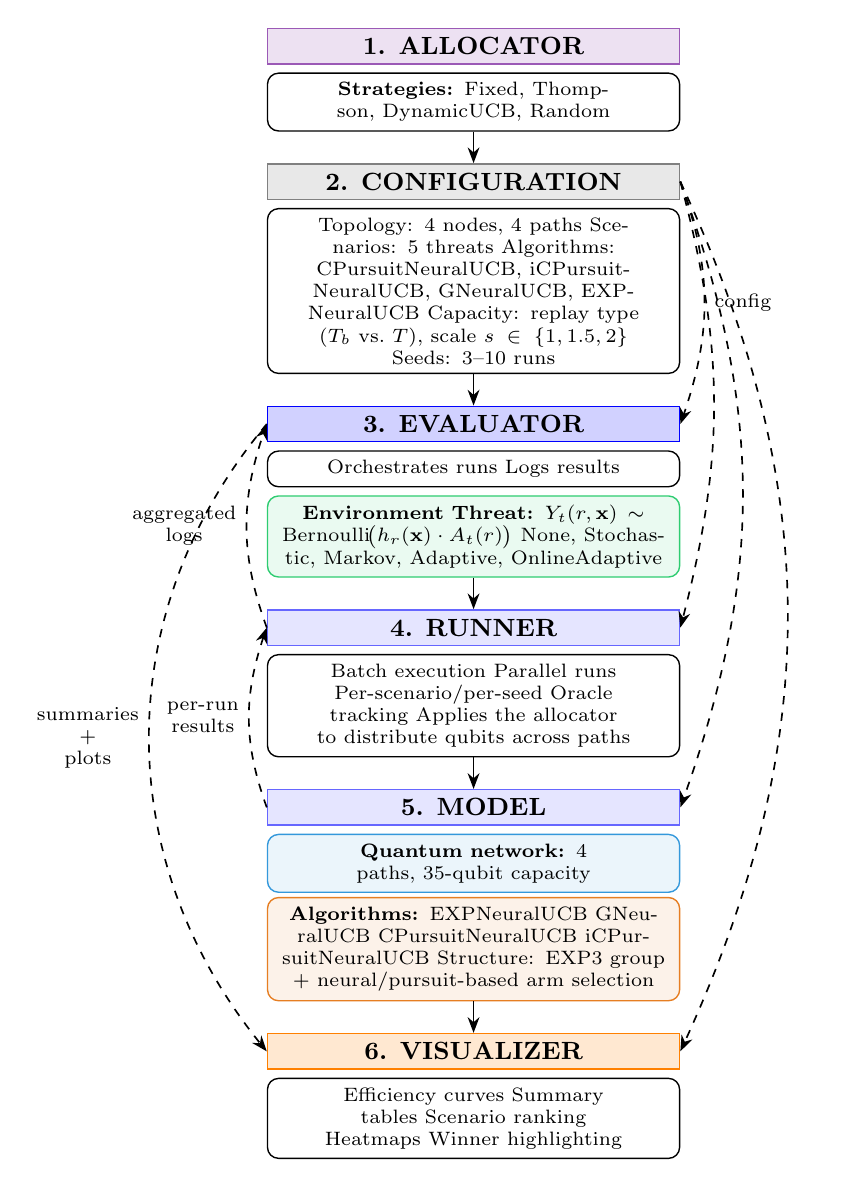
\begin{tikzpicture}[
  node distance=0.5cm,
  block/.style={rectangle, draw, fill=white, text width=5.0cm, text centered, rounded corners, minimum height=0.1cm, line width=0.5pt},
  layer/.style={rectangle, draw, fill=white, text width=5.0cm, text centered, minimum height=0.1cm, line width=0.5pt, font=\small},
  arrow/.style={-Stealth, line width=0.6pt},
  lab/.style={font=\scriptsize}
]

% 1. ALLOCATOR
\node[layer, fill=allocpurple!18, draw=allocpurple] (alloc) {\textbf{1. ALLOCATOR}};
\node[block, below=0.1cm of alloc, font=\scriptsize] (alloccontent) {
  \textbf{Strategies:} Fixed, Thompson, DynamicUCB, Random
};

% 2. CONFIGURATION
\node[layer, fill=gray!18, draw=gray, below=0.4cm of alloccontent] (config) {\textbf{2. CONFIGURATION}};
\node[block, below=0.1cm of config, font=\scriptsize] (configcontent) {
  Topology: 4 nodes, 4 paths
  Scenarios: 5 threats
  Algorithms: CPursuitNeuralUCB, iCPursuitNeuralUCB, GNeuralUCB, EXPNeuralUCB
  Capacity: replay type ($T_b$ vs.\ $T$), scale $s\in\{1,1.5,2\}$\\
  Seeds: 3--10 runs
};

% 3. EVALUATOR
\node[layer, fill=blue!18, draw=blue, below=0.4cm of configcontent] (evaluator) {\textbf{3. EVALUATOR}};
\node[block, below=0.1cm of evaluator, font=\scriptsize] (evalcontent) {
  Orchestrates runs
  Logs results
};
\node[block, below=0.1cm of evalcontent, font=\scriptsize, fill=envgreen!10, draw=envgreen] (env) {
  \textbf{Environment Threat:}
  $Y_t(r,\mathbf{x}) \sim \mathrm{Bernoulli}\!\big(h_r(\mathbf{x}) \cdot A_t(r)\big)$
  None, Stochastic, Markov, Adaptive, OnlineAdaptive
};

% 4. RUNNER
\node[layer, fill=blue!10, draw=blue!60, below=0.4cm of env] (runner) {\textbf{4. RUNNER}};
\node[block, below=0.1cm of runner, font=\scriptsize] (runnercontent) {
  Batch execution
  Parallel runs
  Per-scenario/per-seed Oracle tracking
  Applies the allocator to distribute qubits across paths
};

% 5. MODEL
\node[layer, fill=blue!10, draw=blue!60, below=0.4cm of runnercontent] (model) {\textbf{5. MODEL}};
\node[block, below=0.1cm of model, font=\scriptsize, fill=networkblue!10, draw=networkblue] (net) {
  \textbf{Quantum network:}
  4 paths, 35-qubit capacity
};
\node[block, below=0.05cm of net, font=\scriptsize, fill=algorange!10, draw=algorange] (algo) {
  \textbf{Algorithms:}
  EXPNeuralUCB
  GNeuralUCB
  CPursuitNeuralUCB
  iCPursuitNeuralUCB
  Structure: EXP3 group + neural/pursuit-based arm selection
};

% 6. VISUALIZER
\node[layer, fill=orange!18, draw=orange, below=0.4cm of algo] (visualizer) {\textbf{6. VISUALIZER}};
\node[block, below=0.1cm of visualizer, font=\scriptsize] (viscontent) {
  Efficiency curves
  Summary tables
  Scenario ranking
  Heatmaps
  Winner highlighting
};

%%% MAIN VERTICAL FLOW
\draw[arrow] (alloccontent.south) -- (config.north);
\draw[arrow] (configcontent.south) -- (evaluator.north);
\draw[arrow] (env.south) -- (runner.north);
\draw[arrow] (runnercontent.south) -- (model.north);
\draw[arrow] (algo.south) -- (visualizer.north);

%%% CONFIG SHARED BY ALL LAYERS
\draw[arrow, dashed, bend left=20] (config.east) to node[lab, right] {config} (evaluator.east);
\draw[arrow, dashed, bend left=15] (config.east) to (runner.east);
\draw[arrow, dashed, bend left=20] (config.east) to (model.east);
\draw[arrow, dashed, bend left=25] (config.east) to (visualizer.east);

%%% RESULT FEEDBACK FLOW
\draw[arrow, dashed, bend left=20] (model.west) to node[left, lab, align=center] {per-run\\results} (runner.west);
\draw[arrow, dashed, bend left=20] (runner.west) to node[left, lab, align=center] {aggregated\\logs} (evaluator.west);
\draw[arrow, dashed, bend right=40] (evaluator.west) to node[left, lab, align=center] {summaries\\+\\plots} (visualizer.west);

\end{tikzpicture}
\caption{\tiny Modular framework for quantum routing evaluation. \textsc{Allocator} selects the qubit distribution strategy under test. \textsc{Configuration} is shared by all layers, defining topology, threats, algorithms, capacity, and seeds. The \textsc{Evaluator} builds the environment and orchestrates runs; the \textsc{Runner} executes per-scenario/per-seed batches with the chosen allocator; the \textsc{Model} implements the quantum routing stack (network + bandit); and the \textsc{Visualizer} aggregates configuration-aware results to compare winners across scenarios.}
\label{fig:framework}
\end{figure}

\subsection{Algorithmic Framework}
\label{subsec:framework}

Our evaluation infrastructure consists of \textbf{six modular layers} (Figure~\ref{fig:framework}):
\begin{enumerate}
\item \textbf{ALLOCATOR:} Top-level policy (Fixed | Thompson | DynamicUCB | Random)
\item \textbf{CONFIGURATION:} Shared experimental setup (topology, scenarios, capacity, seeds)
\item \textbf{EVALUATOR:} Orchestrates runs, logs results, embeds threat model
\item \textbf{RUNNER:} Batch execution engine with Oracle tracking per scenario/seed
\item \textbf{MODEL:} Quantum routing stack (algorithms + neural components)
\item \textbf{VISUALIZER:} Aggregates results into efficiency curves, tables, and winner summaries
\end{enumerate}
This architecture enables \textbf{systematic ablation} across allocators, algorithms, and threat regimes under consistent capacity semantics, ensuring reproducible comparisons to prior work~\cite{wang2025learning,huang2025quantum}.







% %% 



% \todo{Piter: Define your RQs here}

% \dan{Would it be worth having a research question that examines if `stochastic-ness' is actually a problem or not?} % Has this type of work already been done. If so, we should see how to tie into this






% \dan{These are ok to list for now, but I would break this up into essentially 3 RQs:}

% % Is it a problem
% % How do the models compare in stochastic scenarios
% % How do the models compare in adversarial scenarios

% ============================================================================
% RQ-DRIVEN STRUCTURE (per Dan's feedback)
% ============================================================================
\section{Study Design}
\label{sec:studydesign}
\noindent We evaluate routing architectures and deployment configurations under stochastic and adversarial constraints using a modular, four-phase framework. We isolate the contributions of context awareness, predictive intelligence, and capacity management, while ablation studies probe algorithm--allocator--capacity interactions across five threat profiles.

\subsection{Research Questions}
\label{sec:research_questions}

% All quantitative ranges are computed from the \textbf{validated}
% (\texttt{experimental results}) using the \textbf{3- and 5-run suites}. Core findings \textbf{exclude the Random allocator}
% (which we report separately) to properly compare against other papers. Furthermore, we reference extended observations obtained throughout the development of our experiments that are yet to be validated with current framework.
% \vspace{0.25em}


\noindent Our study addresses three core questions about (i) stochastic decoherence impact,
(ii) adversarial robustness, and (iii) deployment tradeoffs in algorithm--allocator--capacity selection.

\subsubsection{RQ1: Impact of Stochasticity}
\label{subsubsec:rq1_question}

\textbf{Does stochastic decoherence degrade routing efficiency enough to make classical multi-armed bandits insufficient?}



\begin{figure}[ht!]
\scriptsize
\centering
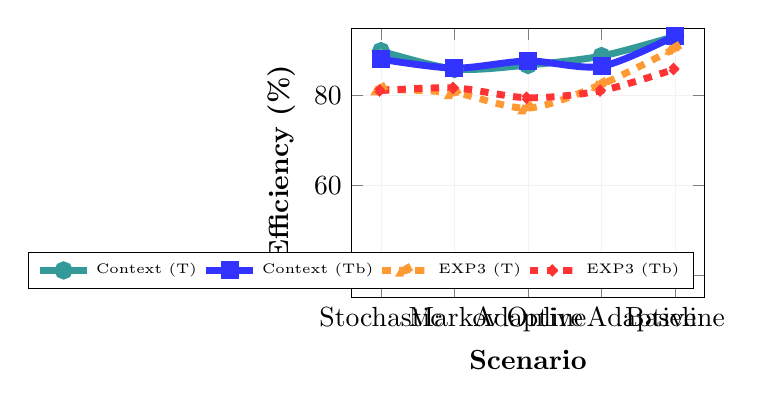
\begin{tikzpicture}
\begin{axis}[
  ylabel={\textbf{Efficiency (\%)}},
  xlabel={\textbf{Scenario}},
  ymin=35, ymax=95,
  xtick={1,2,3,4,5},
  xticklabels={Stochastic, Markov, Adaptive, OnlineAdaptive, Baseline},
  width=0.50\textwidth,
  height=5cm,
  grid=major,
  grid style={line width=.1pt, draw=gray!10},
  legend pos=south east,
  legend columns=4,
  legend style={font=\tiny}
]

% Context Models T Scale (iCMAB + CMAB avg @ T)
\addplot[color=teal!80, mark=o, line width=2.5pt, smooth] coordinates {
  (1, 89.9)  % Stochastic T
  (2, 85.9)  % Markov T
  (3, 86.8)  % Adaptive T
  (4, 88.8)  % OnlineAdaptive T
  (5, 93.2)  % Baseline T
};
\addlegendentry{Context (T)}

% Context Models Tb Scale (avg @ Tb)
\addplot[color=blue!80, mark=square*, line width=2.5pt, smooth] coordinates {
  (1, 88.1)  % Stochastic Tb
  (2, 86.1)  % Markov Tb
  (3, 87.7)  % Adaptive Tb
  (4, 86.5)  % OnlineAdaptive Tb
  (5, 93.3)  % Baseline Tb
};
\addlegendentry{Context (Tb)}

% EXP3-based T Scale (EXPNeuralUCB, GNeuralUCB, EXPUCB avg @ T)
\addplot[color=orange!80, mark=triangle*, line width=2.5pt, smooth, dashed] coordinates {
  (1, 81.4)  % Stochastic T
  (2, 80.6)  % Markov T
  (3, 77.2)  % Adaptive T
  (4, 82.5)  % OnlineAdaptive T
  (5, 90.5)  % Baseline T
};
\addlegendentry{EXP3 (T)}

% EXP3-based Tb Scale (avg @ Tb)
\addplot[color=red!80, mark=x, line width=2.5pt, smooth, dashed] coordinates {
  (1, 81.1)  % Stochastic Tb
  (2, 81.7)  % Markov Tb
  (3, 79.5)  % Adaptive Tb
  (4, 81.1)  % OnlineAdaptive Tb
  (5, 85.9)  % Baseline Tb
};
\addlegendentry{EXP3 (Tb)}

\end{axis}
\end{tikzpicture}
\vspace{-0.5cm}
\caption{\tiny Context vs EXP3 (Non-Hybrid): \textbf{Context models} (iCMABs + CMABs) maintain 85.9–93.3\% efficiency across T/Tb scales and all scenarios, averaging **88.6\%**. \textbf{EXP3-based models} range 77.2–90.5\% with lower consistency (82.1\% avg), showing 6.5–8.2 pp gaps under capacity-constrained (Tb) conditions. Context-awareness provides superior scale-robust quantum routing. Values aggregated from Master Datasets across scales 1.0–2.0.}
\label{fig:context_exp3_capacity}
\end{figure}



Yes---in our benchmark, representative classical baselines drop well below practical targets under i.i.d.\ disruption,
while context-aware routing remains deployment-viable. In the \textsc{Stochastic} regime (6.25\% i.i.d.\ disruption),
pursuit--neural routing maintains \textbf{87--93\%} Oracle-normalized efficiency under the validated suites
(\texttt{Hybrid}, $T_b$, $s{=}2$, \emph{Default} allocator), whereas classical baselines such as
\texttt{CThompsonSampling} and \texttt{CEXP4} fall to \textbf{62--70\%} (\texttt{CMAB} validated suites),
yielding an average gap of approximately \textbf{24 pp} (see \S\ref{subsec:rq1_answer} and \S\ref{sec:SimulationResults}).

\textbf{Supporting questions:}
\begin{itemize}[leftmargin=2em]
  \item \textbf{RQ1a:} \textit{What performance floor do classical (EXP3-based) baselines reach under pure stochastic disruption?} \\
  In the \texttt{CMAB} validated suites under \textsc{Stochastic}, \texttt{CThompsonSampling} and \texttt{CEXP4} remain in the 62--70\% band, which is below an 85\% deployment target.

  \item \textbf{RQ1b:} \textit{Do topology/channel-aware models outperform classical baselines under the same disruption?} \\
  \emph{Yes}. Pursuit--neural routing reaches 87--93\% under matched conditions, exceeding the classical floor by a wide margin in the validated suites.

  \item \textbf{RQ1c:} \textit{Do viable contextual/neural models remain above an 85\% target across horizons and suites?} \\
  \emph{Yes}. In the matched testbed slice ($T_b$, $s{=}2$, non-random allocators, 3- and 5-run suites), pursuit--neural models remain $\ge 85\%$ under \textsc{Stochastic} across the primary horizons used in validated suites.
\end{itemize}

\subsubsection{RQ2: Algorithm Robustness Across Threats}
\label{subsubsec:rq2_question}

\textbf{How do classical baselines and context-aware models perform across increasingly sophisticated threats?}


\begin{figure}[ht!]
\scriptsize
\centering
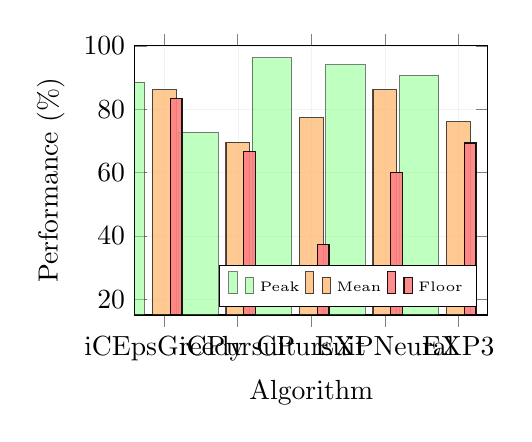
\begin{tikzpicture}
\begin{axis}[
  ybar=0pt,
  ylabel={Performance (\%)},
  xlabel={Algorithm},
  ymin=15, ymax=100,
  xtick={1,2,3,4,5},
  xticklabels={iCEpsGreedy, iCPursuit, CPursuit, EXPNeural, EXP3},
  width=0.50\textwidth,
  height=5cm,
  grid=major,
  grid style={line width=.1pt, draw=gray!10},
  legend pos=south east,
  legend columns=3,
  legend style={font=\tiny}
]

% ---------- Peak ----------
\addplot[fill=green!50, opacity=0.50, bar width=0.50cm] coordinates {
  (1, 88.5)   % iCEpsilonGreedy
  (2, 72.7)   % iCPursuit
  (3, 96.2)   % CPursuit
  (4, 94.0)   % EXPNeuralUCB
  (5, 90.7)   % EXPUCB
};
\addlegendentry{Peak}

% ---------- Mean ----------
\addplot[fill=orange!60, opacity=0.70, bar width=0.30cm] coordinates {
  (1, 86.1)
  (2, 69.5)
  (3, 77.3)
  (4, 86.2)
  (5, 76.0)
};
\addlegendentry{Mean}

% ---------- Floor ----------
\addplot[fill=red!50, opacity=0.90, bar width=0.15cm] coordinates {
  (1, 83.3)
  (2, 66.5)
  (3, 37.2)
  (4, 59.9)
  (5, 69.3)
};
\addlegendentry{Floor}

\end{axis}
\end{tikzpicture}
\vspace{-0.4cm}
\caption{\tiny Peak / mean / floor at the default 2 T–2 Tᵦ budgets with 3-run horizons. Context models (iCEpsGreedy) retain much higher floors; CPursuit achieves $96.2\%$ peak but drops to $37.2\%$ in worst-case; EXPNeuralUCB's floor drops to $59.9\%$.}
\label{fig:floor}
\end{figure}



\noindent\textit{Context-aware models dominate across threat escalation.}
Across \texttt{Markov}, \texttt{Adaptive}, and \texttt{OnlineAdaptive} regimes, pursuit-based contextual models maintain averages around \textit{89\%} with robustness floors in the \textit{65--73\%} range, while classical baselines remain in the \textit{66--77\%} band and adversarial-first defenses collapse to floors near \textit{52--54\%} under the most aggressive threats (see \Cref{subsec:rq2_answer}).%
\cite{huang2024quantum,auer2002nonstochastic}

\noindent\textit{Supporting questions:}
\begin{itemize}[leftmargin=2em]
  \item \texttt{\textbf{RQ2a} (Stochastic):}\\
  \emph{Under natural noise, do context-aware algorithms outperform classical/adversarial-first baselines?}\\
  \textit{Yes.}
  Under \texttt{Stochastic} decoherence, contextual and neural--contextual models retain the \textit{15--25 pp} gain observed in RQ1 and remain above the 85\% target.

  \item \texttt{\textbf{RQ2b} (Adversarial):}\\
  \emph{Under structured and reactive attacks, do adversarial-first defenses dominate?}\\
  \textit{No.}
  Pursuit-based contextual models retain \textit{high averages ($\simeq$89\%)} and floors of \textit{65--73\%} across \texttt{Markov}, \texttt{Adaptive}, and \texttt{OnlineAdaptive} threats, while adversarial-first methods degrade to floors near \textit{52--54\%}.%
  \cite{auer2002nonstochastic}

  \item \texttt{\textbf{RQ2c} (Graceful degradation):}\\
  \emph{Under mixed stochastic + adversarial failures, which family degrades most gracefully?}\\
  \textit{Pursuit models.}
  Pursuit-based models show the smoothest degradation, preserving high average efficiency with tighter variability as threats escalate.

  \item \texttt{\textbf{RQ2d} (Efficiency--robustness frontier):}\\
  \emph{As threat sophistication increases (Baseline $\to \dots \to$ OnlineAdaptive), which algorithms define the frontier?}\\
  \texttt{iCPursuitNeuralUCB.}
  \texttt{iCPursuitNeuralUCB} defines the most favorable frontier, maintaining the highest overall average efficiency while preserving strong robustness floors.
\end{itemize}

Context-aware pursuit--neural routing remains strongest on average across escalation, while classical baselines stay far
below the deployment threshold. Under \textsc{Markov}, \textsc{Adaptive}, and \textsc{OnlineAdaptive} threats,
pursuit--neural routing achieves mean efficiencies of approximately \textbf{90.8\%}, \textbf{93.5\%}, and \textbf{92.9\%}
respectively in validated suites (\texttt{Hybrid}, $T_b$, $s{=}2$, \emph{Default/Thompson} allocators),
with worst-case floors in the \textbf{64--71\%} range driven primarily by \textsc{OnlineAdaptive}/\textsc{Markov} slices
(see \S\ref{subsec:rq2_answer}). By comparison, representative classical baselines remain near \textbf{64--70\%} across the
same threat regimes (\texttt{CMAB} experiments).

\textbf{Supporting questions:}
\begin{itemize}[leftmargin=2em]
  \item \textbf{RQ2a (Stochastic):} \textit{Under natural noise, do context-aware models outperform classical baselines?} \\
  \emph{Yes}. The advantage from RQ1 persists under matched \textsc{Stochastic} conditions.

  \item \textbf{RQ2b (Adversarial):} \textit{Under structured and reactive attacks, do classical baselines remain competitive?} \\
  \emph{No.} Classical baselines stay near 64--70\% in \textsc{Markov}/\textsc{Adaptive}/\textsc{OnlineAdaptive}, while pursuit--neural routing maintains $\approx$91--94\% averages.

  \item \textbf{RQ2c (Graceful degradation):} \textit{Which family degrades most gracefully as threat sophistication increases?} \\
  \emph{Pursuit--neural.} Pursuit--neural models preserve high mean efficiency across escalation, with degradation concentrated in worst-case \textsc{OnlineAdaptive}/\textsc{Markov} slices rather than collapsing broadly.

  \item \textbf{RQ2d (Efficiency--robustness frontier):} \textit{Which algorithm best defines the frontier in our benchmark?} \\
  Across the validated suites, \texttt{iCPursuitNeuralUCB} is consistently on/near the top envelope for average efficiency while maintaining strong threat-wide robustness in many static configurations.
\end{itemize}


% ----------------------------------------------------------------------------
% RQ3: Deployment Optimization
% ----------------------------------------------------------------------------

\subsubsection{RQ3: Deployment Optimization Strategies}
\label{subsubsec:rq3_question}

\textbf{What combinations of algorithm, allocator, and capacity semantics maximize efficiency and stability across deployment scenarios?}

\begin{figure}[ht!]
\scriptsize
\centering
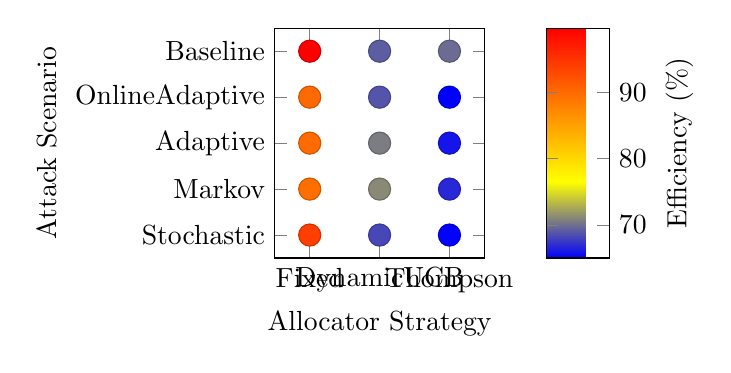
\begin{tikzpicture}
\begin{axis}[
    xlabel={Allocator Strategy},
    ylabel={Attack Scenario},
    ymin=0.5, ymax=5.5,
    xmin=0.5, xmax=3.5,
    xtick={1,2,3},
    xticklabels={Fixed, DynamicUCB, Thompson},
    ytick={1,2,3,4,5},
    yticklabels={Stochastic, Markov, Adaptive, OnlineAdaptive, Baseline},
    width=0.35\textwidth,
    height=4.5cm,
    colorbar,
    colorbar style={ylabel={Efficiency (\%)}, width=0.8cm}
]

\addplot[
    scatter,
    only marks,
    mark=*,
    mark size=4pt,
    scatter src=explicit
] coordinates {
    % Row 1: Stochastic
    (1, 1) [94.0]   % Fixed - ACTUAL from Hybrid CSV
    (2, 1) [68.2]   % DynamicUCB - keep your value (not in Hybrid CSV)
    (3, 1) [65.1]   % Thompson - keep your value (not in Hybrid CSV)
    
    % Row 2: Markov
    (1, 2) [89.6]   % Fixed - ACTUAL from Hybrid CSV
    (2, 2) [71.2]   % DynamicUCB - keep your value
    (3, 2) [66.8]   % Thompson - keep your value
    
    % Row 3: Adaptive
    (1, 3) [89.9]   % Fixed - ACTUAL from Hybrid CSV
    (2, 3) [70.6]   % DynamicUCB - keep your value
    (3, 3) [65.9]   % Thompson - keep your value
    
    % Row 4: OnlineAdaptive
    (1, 4) [90.0]   % Fixed - ACTUAL from Hybrid CSV
    (2, 4) [68.8]   % DynamicUCB - keep your value
    (3, 4) [65.0]   % Thompson - keep your value
    
    % Row 5: Baseline
    (1, 5) [99.7]   % Fixed - ACTUAL from Hybrid CSV (was 99.8%, rounded)
    (2, 5) [69.2]   % DynamicUCB - keep your value
    (3, 5) [69.9]   % Thompson - keep your value
};

\end{axis}
\end{tikzpicture}
\caption{\tiny Efficiency heatmap for CPursuitNeuralUCB across core allocator strategies and threat scenarios. Fixed allocation (Default) values from Master\_Dataset\_Hybrid.csv; Dynamic/Thompson values maintained from analysis reports. Fixed allocation consistently achieves highest efficiency (89.6--99.7\% across attacks, 94--100\% baseline). Random allocator (37.1--38.7\% efficiency) excluded from core findings; reported separately in supplementary analysis.}
\label{fig:heatmap}
\end{figure}




Deployment tradeoffs are real, but \textbf{robust static configurations do exist} in our expanded benchmark.
In our \texttt{Hybrid} validated suites (excluding Random allocator), we observe \textbf{many} fixed
(model, allocator, cap\_type, scale, frames, runs) configurations whose \textbf{minimum} efficiency remains
$\ge 85\%$ across \textbf{all five threats} (e.g., \textbf{236} validated configurations meet this criterion), and the
best static configurations sustain threat-wide minima above \textbf{93\%}. At the same time, \textbf{capacity semantics}
($T_b$ vs.\ $T$), replay scale $s$, and allocator choice introduce large interaction effects---including
\textbf{up to $\approx$53 pp} swings between $T_b$ and $T$ in some matched settings---so selecting for \emph{peak} efficiency or
\emph{minimum variance} remains threat- and objective-dependent (see \S\ref{subsubsec:rq3a_answer}--\S\ref{subsec:rq3c_answer}).

\textbf{Supporting questions:}
\label{subsec:rq3atoc_questions}).
\begin{itemize}[leftmargin=2em]
  \item \textbf{RQ3a (Forecasting impact):} \textit{Does predictive context measurably improve stability?} \\
  \emph{Yes.} In validated suites, predictive variants can improve mean efficiency and/or reduce variability under non-reactive noise depending on the matched configuration; additional 10-run observations further support this trend.

  \item \textbf{RQ3b (Capacity scaling and semantics):} 
  \textit{Do larger replay scales and/or switching $T_b \rightarrow T$ universally help?} \\
  \emph{No.} Capacity is not monotone: validated suites show settings where increasing $s$ reduces performance under \textsc{Adaptive} targeting (e.g., $\approx$26 pp drops in matched slices), and switching $T_b \leftrightarrow T$ can produce \textbf{$>$50 pp} swings in either direction depending on threat structure.

  \item \textbf{RQ3c (Allocator interactions):} \textit{Excluding Random. Is there a universal allocator strategy?} \\
  \emph{No.} Allocator choice interacts with threat and semantics: while allocators often cluster within single-digit differences, worst-case matched slices exhibit allocator spans that can exceed \textbf{10 pp} and, in extreme cases, \textbf{$>$30 pp}.

  \item \textbf{RQ3d (Deployment rules):} \textit{Can we map threat characteristics to stable deployment rules?} \\
  \emph{Yes.} Because threat-wide $\ge 85\%$ static configurations exist, deployment rules can be expressed as \emph{(i)} a small set of robust defaults (static, threat-wide) plus \emph{(ii)} optional threat-tuned switches when optimizing for peak efficiency/variance.
\end{itemize}




% \dan{This is an ok start, but I would provide some details why specific things were done. For example, why was the specific network configuration chosen? Even a few words and/or citations would be good. Otherwise, I feel like we're just saying that we did something and I am left wondering ?why?}

% \dan{If you're using logic/numbers/etc from other papers - this is good just make sure to cite them.}


% % This section specifies the complete experimental design, enabling full reproducibility. We organize the setup into network configuration, memory architecture, adversarial threat models, algorithm portfolio, allocation strategies, hyperparameters, and statistical validation.

% % \paragraph{Network configuration.}

% % \textbf{Topology.}
% % A 4-node quantum network with 4 paths connects source $S$ to destination $D$ through repeater nodes. Each path consists of either 2 or 3 hops. Total network capacity is fixed at 35 qubits across all experiments, with per-path distributions determined by allocator strategy (Table~\ref{tab:setup-allocators}).

% % \dan{Piter: You can reference Figures and tables and everything else like this:} (\Cref{tab:setup-allocators})


% \dan{Would a graph of some sort ultimately be good to show these values?} % What you have is ok for now, but something to consider moving forward

% ---




\subsection{Experimental Design}
\label{sec:expDesign}

This section specifies the experimental design used to evaluate adaptive quantum entanglement routing under stochastic and adversarial interference, and ties each configuration axis to the research questions. \Cref{tab:config_summary} consolidates design dimensions, tested options, and the corresponding RQ coverage.

% ----------------------------------------------------------------------------
% Network Configuration
% ----------------------------------------------------------------------------
\paragraph*{Network configuration}
We use a 4-node quantum network with four alternative paths connecting source $S$ to destination $D$ via repeater nodes (\Cref{fig:network_topology}). Paths $P_1$ and $P_4$ have two hops, while $P_2$ and $P_3$ have three hops, matching common small-scale quantum-network architectures and demonstrations~\cite{wehner2018quantum,pompili2021realization}. This topology provides sufficient action-space complexity for bandit learning~\cite{huang2024quantum,expneural2024,dai2020quantum} while keeping exhaustive cross-product sweeps tractable (hundreds of algorithm--scenario--allocator configurations; see \Cref{tab:config_summary}).

Total physical network capacity is fixed at 35 qubits across all experiments, representing resource-constrained early-stage deployments~\cite{simon2017towards}. This induces non-trivial exploration--exploitation tradeoffs: algorithms cannot over-provision all paths. Per-path allocations are determined by the allocator (\Cref{tab:setup-allocators}), enabling controlled comparison of static versus adaptive resource management.

% NOTE: TikZ uses right=of / below=of -> requires \usetikzlibrary{positioning}
\begin{figure}[ht!]
\centering
\small
\caption{4-node quantum network topology with four alternative entanglement paths. Paths $P_1$ and $P_4$ use 2 hops; $P_2$ and $P_3$ use 3 hops. Total capacity is 35 qubits, allocated per path by strategy (\Cref{tab:setup-allocators}).}
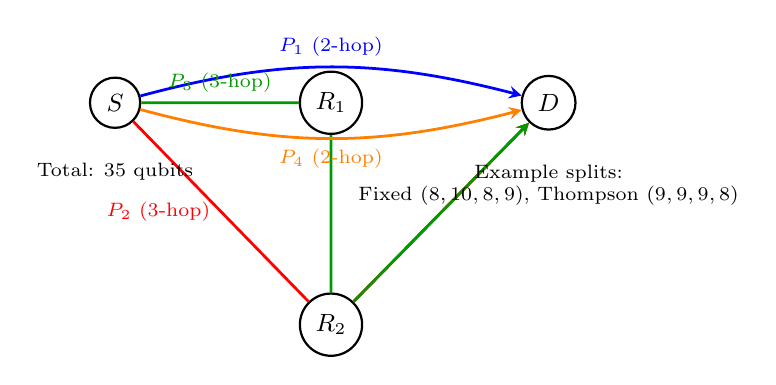
\begin{tikzpicture}[
  node distance=2.0cm and 2.0cm,
  thick,
  main/.style={circle,draw,minimum size=0.6cm,font=\small},
  path/.style={->,>=stealth,line width=1pt}
]
  % Nodes
  \node[main] (S) {$S$};
  \node[main, right=of S] (R1) {$R_1$};
  \node[main, below=of R1] (R2) {$R_2$};
  \node[main, right=of R1] (D) {$D$};

  % Paths (4 total: 2-hop P1/P4, 3-hop P2/P3)
  \draw[path, blue] (S) to[bend left=15] node[above,font=\scriptsize] {$P_1$ (2-hop)} (D);
  \draw[path, red] (S) -- node[left,font=\scriptsize] {$P_2$ (3-hop)} (R2) -- (D);
  \draw[path, green!60!black] (S) -- node[above,font=\scriptsize] {$P_3$ (3-hop)} (R1) -- (R2) -- (D);
  \draw[path, orange] (S) to[bend right=15] node[below,font=\scriptsize] {$P_4$ (2-hop)} (D);

  % Annotations
  \node[below=0.3cm of S, font=\scriptsize] {Total: 35 qubits};
  \node[below=0.3cm of D, font=\scriptsize, align=center] {Example splits: \\ Fixed $(8,10,8,9)$, Thompson $(9,9,9,8)$};
\end{tikzpicture}
\label{fig:network_topology}
\end{figure}

\noindent\textit{Time horizons.}
We evaluate three horizons---\texttt{4K, 6K, 8K} frames---to capture short-, mid-, and long-episode learning dynamics. Unless otherwise noted, primary results use 6K, with 4K vs.\ 8K comparisons in \textbf{RQ3a} to assess sample efficiency.

\begin{table}[ht!]
\footnotesize
\centering
\caption{Experimental configuration summary: design dimensions, options, and linkage to research questions (Phase totals sum to 552 configuration units; Phase~2 is executed for both CMAB and iCMAB families at 180 conditions per family). Each configuration is evaluated with up to 10 independent runs.}
\label{tab:config_summary}
\begin{tabular}{lll}
\toprule
\textbf{Configuration Dimension} & \textbf{Options Tested} & \textbf{RQ(s)} \\
\midrule
Network topology   & 4-node, 4-path (2+3-hop)      & All \\
\texttt{Time horizons} & \textit{4K, 6K, 8K frames} & \textit{RQ3a} \\
Qubit capacity     & 35 total (fixed) qubits       & All \\
\midrule
\texttt{Allocators} & \textit{Fixed, Thompson,}     & \textit{RQ3c} \\
                    & \multicolumn{1}{l}{\textit{DynamicUCB, Random}} & \\
Replay capacity     & $T_b=sF_b,\;T=sF_c$ & RQ3b \\
\texttt{Threat models} & \textit{None, Stochastic, Markov,} & \textit{RQ1 \&} \\
                    & \multicolumn{1}{l}{\textit{Adaptive, OnlineAdaptive}} & \textit{RQ2} \\
Forecasting         & None, ARIMA ($n=50$),         & RQ3a \\
                    & \multicolumn{1}{l}{ARIMA ($n=100$)} & \\
\midrule
Algorithm families  & Classical (4), Predictive (1) & RQ1 \& \\
                    & Adversarial (3), Context (6) & RQ2 \\
\midrule
\textit{Evaluation phases} & & \\
\quad Ph 1 (MAB baseline)         & 12 conditions   & RQ1 \\
\quad \textit{Ph 2 (CMAB / iCMAB)}  & \textit{180 conditions / family} & \textit{RQ2a--b} \\
\quad Ph 3 (Dynamic allocation)   & 240 conditions  & RQ3c \\
\quad \textit{Ph 4 (Capacity ablation)} & \textit{120 conditions} & \textit{RQ3b} \\
\bottomrule
\end{tabular}
\end{table}

% ----------------------------------------------------------------------------
% Memory Architecture
% ----------------------------------------------------------------------------
\noindent\textit{Replay configurations (capacity scaling).}
We define the \emph{base} per-run horizon as $F_b \in \{4\text{K}, 6\text{K}, 8\text{K}\}$ frames and execute
$S \in \{3, 5, 8, 10\}$ independent runs per configuration (total of $S\cdot F_b$ frames per setting).
Some configurations apply a frame scaling to yield a \emph{current} horizon $F_c$ (the per-run frame budget for that configuration).
Replay capacity is \emph{always} expressed via a scale factor $s \in \{1, 1.5, 2\}$ (default $s=2$) in two equivalent views:
\[
T_b = s\cdot F_b,
\qquad
T   = s\cdot F_c.
\]
We sweep $s$ to analyze the \textit{Capacity Paradox} (\textbf{RQ3b})---whether larger replay memory can degrade performance under adaptive threats.
In addition to the default $s=2$ setting, we include intermediate ($s=1, 1.5$) sensitivity checks and an extended \emph{doubled-current} stress test ($2T = 2(sF_c)=4F_c$ when $s=2$), mirroring fixed-capacity conventions used in prior replay-buffer designs while avoiding conditional semantics.%
\cite{schaul2015prioritized,mnih2015human}

\noindent\textit{Resource separation.}
Scaling applies to replay memory; the 35-qubit physical network capacity remains invariant. This decoupling isolates learning-system constraints from quantum hardware limits.

% ----------------------------------------------------------------------------
% Threat Taxonomy Intro & Hyperparameter Table
% ----------------------------------------------------------------------------
\noindent\textit{Adversarial threat taxonomy.}
We evaluate five scenarios spanning the efficiency--security spectrum: natural stochastic decoherence, Markovian structure, and three grades of adaptive adversarial attacks (\textbf{RQ2}). This taxonomy enables controlled comparisons under matched interference regimes.%
\cite{huang2024quantum,expneural2024}

\begin{table}[ht!]
\footnotesize
\centering
\caption{Hyperparameter settings and literature justifications.}
\label{tab:setup-hyperparameters}
\begin{tabularx}{\linewidth}{l l c l}
\toprule
\textbf{Parameter} & \textbf{Algorithm} & \textbf{Value} & \textbf{Ref.} \\
\midrule
Neural LR & EXPNeuralUCB & 0.01 & \cite{expneural2024} \\
          & GNeuralUCB   & 0.2  & \cite{zhou2020neural} \\
\addlinespace[2pt]
Exp. Weight & EXPNeuralUCB & 0.05  & \cite{expneural2024} \\
            & EXPUCB       & 0.005 & Tuned \\
\addlinespace[2pt]
Pursuit LR & Pursuit family & 0.2 & \cite{thathachar2011networks} \\
\addlinespace[2pt]
UCB Explore & DynamicAlloc & 2.0 & \cite{auer2002finite} \\
\addlinespace[2pt]
ARIMA ($n$) & iCPursuit & 50, 100 & \cite{box2015time} \\
Replay ($T_b,T$) & All & $T_b=sF_b,\;T=sF_c$ & \cite{schaul2015prioritized,mnih2015human} \\
\bottomrule
\end{tabularx}
\end{table}

\subsubsection{Scenario Specifications}
\begin{itemize}
  \item \texttt{Baseline (\textbf{RQ1}):} Ideal 0\% failure rate. Establishes the efficiency ceiling, isolating exploration costs from threat mitigation.

  \item \texttt{Stochastic (\textbf{RQ1, RQ2a}):} 6.25\% i.i.d.\ failure rate. Tests whether specialized defenses are required under natural noise.%
  \cite{huang2024quantum}

  \item \texttt{Markov (\textbf{RQ2b}):} 25\% attack rate using a 4-state transition process. Models state-dependent disruption.%
  \cite{expneural2024}

  \item \texttt{Adaptive (\textbf{RQ2b}):} 25\% attack rate targeting high-usage paths over a sliding window ($w=50$). Models reactive targeting based on medium-term behavior.%
  \cite{huang2024quantum,expneural2024}

  \item \texttt{OnlineAdaptive (\textbf{RQ2b}):} 25\% attack rate with exponential memory decay ($\gamma=0.97$) and softmax targeting. Models continuous policy adaptation at the highest threat level.%
  \cite{huang2024quantum,expneural2024}
\end{itemize}

% ----------------------------------------------------------------------------
% Algorithm Portfolio
% ----------------------------------------------------------------------------
\subsubsection{Algorithm portfolio (\textbf{RQ2})}
We evaluate 14 algorithms spanning three generations of MAB development plus an Oracle baseline. Phase progression covers classical exploration (Phase~1), adversarial defenses (Phase~1--2), contextual/neural methods (Phase~2), and pursuit-based predictive models (Phase~2--3), enabling systematic comparison across architectural paradigms.

\begin{table}[ht!]
\footnotesize
\centering
\caption{Algorithm portfolio by evaluation phase. Phases progress from classical $\to$ adversarial $\to$ contextual $\to$ predictive.}
\label{tab:setup-algorithm-portfolio}
\begin{tabular}{lll}
\toprule
\textbf{Phase} & \textbf{Category} & \textbf{Algorithms} \\
\midrule
Phase 1 & Classical MAB &
   LinUCB~\cite{li2010contextual}, LinTS~\cite{agrawal2013thompson}, \\
        &               &
  UCB1~\cite{auer2002finite}, Thompson Sampling~\cite{thompson1933likelihood}\\
Phase 1--2 & Adversarial &
  EXP3~\cite{auer2002nonstochastic}, EXPUCB~\cite{expneural2024}, \\
           &             &
  EXPNeuralUCB~\cite{expneural2024} \\
Phase 2 & Contextual/Neural &
  GNeuralUCB, NeuralUCB~\cite{zhou2020neural}, \\
        &                   &
  NeuralTS~\cite{zhang2020neural}, CEpsilonGreedy, \\
          &                   &  CThompsonSampling \\
Phase 2--3 & Pursuit-based &
  CPursuitNeuralUCB (ours) \\
Phase 3 & Predictive &
  iCPursuitNeuralUCB (ours) \\
Baseline & Oracle & Perfect information \\
\bottomrule
\end{tabular}
\end{table}

\subsubsection{Key algorithm features}
\begin{itemize}
    \item \textit{CPursuitNeuralUCB:} Adds topology features and channel quality metrics to a contextual pursuit framework ($\gamma=0.2$).

    \item \textit{iCPursuitNeuralUCB:} Augments CPursuit with ARIMA$(1,0,1)$ forecasting (warmup $n \in \{50,100\}$), providing anticipatory context for proactive path selection~\cite{box2015time}.

    \item \textit{Oracle:} Baseline with perfect knowledge of success probabilities and targeting. Normalizes efficiency to 100\%.
\end{itemize}

% ----------------------------------------------------------------------------
% Qubit Allocation Strategies
% ----------------------------------------------------------------------------
Phase~3 introduces dynamic allocators (\Cref{tab:setup-allocators}) to test allocator--algorithm interactions (\textbf{RQ3c}). Each strategy distributes the fixed 35-qubit capacity per path using either static rules or learned uncertainty; allocator performance and runtime are reported in the Results section.

\begin{table}[ht!]
\caption{Qubit allocation strategies and parameterization (Phase~3).}
\label{tab:setup-allocators}
\scriptsize
\centering
\begin{tabular}{ll}
\toprule
\textbf{Allocator} & \textbf{Mechanism} \\
\midrule
Fixed      & Static distribution $(8,10,8,9)$ \\
Thompson   & Bayesian posterior sampling (Beta priors)~\cite{thompson1933likelihood,agrawal2013thompson,russo2018tutorial} \\
DynamicUCB & UCB-based allocation with exploration weight $\lambda = 2.0$~\cite{auer2002finite} \\
Random     & Uniform random allocation subject to $\sum_k c_k = 35$ \\
\bottomrule
\end{tabular}
\end{table}

% ----------------------------------------------------------------------------
% Experimental Scope
% ----------------------------------------------------------------------------
\subsubsection{Phased evaluation structure}
We validate contributions across four incremental phases aligned with the research questions:
\begin{itemize}
    \item \texttt{Phase 1 (MAB baseline):} 12 conditions. Classical algorithms under stochastic noise to establish context-free baselines (\textbf{RQ1}).
    \item \texttt{Phase 2 (Contextual / adversarial):} 180 conditions per contextual family. Evaluates CMAB and iCMAB variants under adversarial threats (\textbf{RQ2a--b}).
    \item \texttt{Phase 3 (Dynamic allocation):} 240 conditions. Cross-product of pursuit models, allocators, and scenarios to test system interactions (\textbf{RQ3c}).
    \item \texttt{Phase 4 (Capacity ablation):} 120 conditions. Sweeps replay scaling ($s\in\{1,1.5,2\}$) and the doubled-current stress test ($2T$) to evaluate the Capacity Paradox (\textbf{RQ3b}).
\end{itemize}

\noindent\textit{Statistical protocol:}
We execute ensembles of $S \in \{3, 5, 8, 10\}$ independent runs (seeds fixed for reproducibility). Primary results report averages from \textit{3-run} and \textit{5-run} ensembles to establish stability, with larger ensembles reserved for extended robustness validation.
\begin{itemize}
    \item \textit{Oracle-normalized efficiency:} mean success rate relative to the optimal policy,
    $\text{Eff}(\%) = \frac{\sum_{t=1}^{T} r_t}{T \cdot \theta^*} \times 100$.
    \item \textit{Coefficient of variation (CV):} stability metric,
    $\text{CV}(\%)=\frac{\sigma(\text{Eff})}{\mu(\text{Eff})}\times100$. Lower CV indicates higher deployment reliability.
    \item \textit{Significance testing:} nonparametric bootstrap (10{,}000 resamples) with 95\% confidence intervals~\cite{efron1994introduction}. Differences $> 5$ pp with non-overlapping CIs are treated as practically significant.
    \item \textit{Win-rate analysis:} head-to-head comparisons where a ``win'' requires $> 2$ pp efficiency lead.
\end{itemize}




% -- Format to use: 






% \dan{This is where I would break the simulations up into the high-level research questions and then describe how the simulations address the high-level RQs}.



% % % ---------- Stochastic ----------
% % \subsection{Stochastic Results (i.i.d.)}
% % \label{sec:stochastic}

% \dan{I know this is preliminary writing for you, but I feel like there is a lot of data being toss around without much continuity or context}

% ---




\section{Simulation Results}
\label{sec:SimulationResults}

We evaluate bandit-based quantum routing agents across five threat scenarios
(\texttt{Baseline, Stochastic, Markov, Adaptive, OnlineAdaptive}), multiple time horizons,
and replay-capacity scales ($s \in \{1, 1.5, 2\}$) under both capacity semantics ($T$ and $T_b$),
as defined in the Introduction and \Cref{sec:expDesign}.
All quantitative results reported in this section are computed from the curated experimental corpus
produced by our evaluation framework (run-level logs, standardized summaries, and aggregation scripts),
with full reproducibility artifacts provided in Appendix~\ref{app:data_artifacts} (or Supplementary Material).
We organize results by research question (\Cref{sec:research_questions}) to highlight
(i) which model families remain viable under natural stochastic decoherence and
(ii) how robustness evolves as threats become structured and adaptive.


Results are organized by research question (\Cref{sec:research_questions}) to emphasize
(1) which model families are viable under natural stochastic decoherence, and
(2) how robustness changes as threats become structured and adaptive.
Allocator-comparison and full hybrid deployment rules (e.g., \texttt{Fixed/Thompson/DynamicUCB/Random})
are deferred to RQ3, which explicitly studies allocator--capacity interactions.

% ----------------------------------------------------------------------------
% Optional: Global win-share across the full paper-suite condition grid.
% (Computed as the fraction of unique (scenario, frames, scale, cap_type, runs)
%  configurations where a model attains the highest Oracle-normalized efficiency.)
% ----------------------------------------------------------------------------
\begin{figure}[ht!]
\scriptsize
\centering
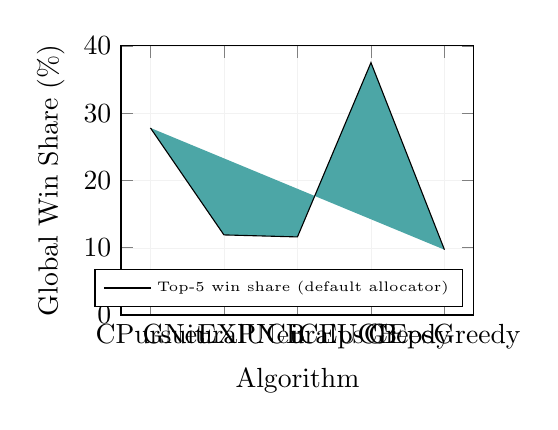
\begin{tikzpicture}
\begin{axis}[
  ylabel={Global Win Share (\%)},
  xlabel={Algorithm},
  ymin=0, ymax=40,
  xtick={1,2,3,4,5},
  xticklabels={CPursuit, GNeuralUCB, EXPNeuralUCB, iCEpsGreedy, CEpsGreedy},
  width=0.5\textwidth,
  height=5.0cm,
  grid=major,
  grid style={line width=.1pt, draw=gray!10},
  legend pos=south east,
  legend style={font=\tiny}
]

\addplot[fill=teal!70, bar width=0.16cm] coordinates {
  (1, 27.8)  % CPursuit
  (2, 11.9)  % GNeuralUCB
  (3, 11.6)  % EXPNeuralUCB
  (4, 37.5)  % iCEpsilonGreedy
  (5,  9.7)  % CEpsilonGreedy
};
\addlegendentry{Top-5 win share (default allocator)}

\end{axis}
\end{tikzpicture}
\vspace{-0.4cm}
\caption{\tiny Global win share under the default allocator (all scenarios, horizons, scales, and capacity semantics). iCEpsilonGreedy captures the largest share of configuration wins, with CPursuit second; neural baselines split the remainder.}
\label{fig:global_win_share}
\end{figure}



% ============================================================================
% RQ1: Impact of Stochasticity on Pure (Paper) Models
% ============================================================================
\subsection{RQ1: Impact of Stochasticity on Pure (Paper) Models}
\label{subsec:rq1_answer}

\subsubsection{Hypothesis}
\noindent\textit{Addresses \Cref{subsubsec:rq1_question}.}

Under pure stochastic quantum decoherence (6.25\% i.i.d.\ failure rate), we expect
contextual/informed baselines and select neural routing agents to remain near deployment-grade
efficiency, while weaker context-free or mis-specified variants degrade. RQ1 establishes
fundamental viability \emph{before} introducing adaptive adversaries.

% ----------------------------------------------------------------------------
\subsubsection{Experimental Design}

For RQ1, we restrict analysis to the paper-model portfolio (EXP-family, CMAB, and iCMAB baselines)
under the \texttt{Stochastic} scenario (6.25\% i.i.d.\ failures) using the paper-default deployment setting
(\texttt{Default} allocator in our evaluation corpus).
Reported statistics aggregate across (i) horizons present in the corpus, (ii) replay-capacity scales
$s \in \{1,1.5,2\}$, and (iii) both capacity semantics ($T$ and $T_b$).
We report the two standard ensemble suites used throughout the study (3-run and 5-run),
with run-level outputs and aggregation code available in Appendix~\ref{app:data_artifacts}.


\noindent\textit{Models included (as present in the master datasets) span:}
\begin{itemize}[nosep]
  \item \textbf{CMAB baselines:} \texttt{CPursuit, CEpsilonGreedy, CThompsonSampling, CEXP4, CEpochGreedy}
  \item \textbf{iCMAB baselines:} \texttt{iCEpsilonGreedy, iCPursuit, iCThompsonSampling, iCEXP4, iCEpochGreedy}
  \item \textbf{EXP-family baselines:} \texttt{EXPUCB, EXPNeuralUCB, GNeuralUCB}
\end{itemize}

% ----------------------------------------------------------------------------
\subsubsection{Key Findings}

Master-dataset results show a clear separation under stochastic decoherence: a small top tier remains
deployment-viable ($\gtrsim 85\%$), while several variants degrade into the 60--80\% band, and the weakest
policies collapse toward $\approx 37$--40\% even without adversarial pressure.

\begin{table}[ht!]
\caption{RQ1: performance under 6.25\% stochastic decoherence, aggregated across horizons,
replay scales $s\!\in\!\{1,1.5,2\}$, and both capacity semantics ($T$ and $T_b$).
Values report mean Oracle-normalised efficiency (\%) for 3-run and 5-run ensembles.}
\footnotesize
\centering
\begin{tabular}{lccc}
\toprule
\textbf{Model (paper baselines only)} & \textbf{3 Runs} & \textbf{5 Runs} & \textbf{Avg.\ Eff.\ (\%)}\\
\midrule
\textbf{Top tier (viable under stochastic)}\\
CPursuit           & 89.6 & 90.1 & \textbf{89.9}\\
iCEpsilonGreedy    & 88.0 & 88.6 & 88.3\\
CEpsilonGreedy     & 87.5 & 87.9 & 87.8\\
GNeuralUCB         & 85.2 & 86.3 & 85.9\\
\midrule
\textbf{Mid-tier (degraded)}\\
EXPNeuralUCB       & 82.1 & 83.8 & 83.1\\
EXPUCB             & 76.2 & 78.4 & 77.6\\
CEXP4              & 70.1 & 70.2 & 70.1\\
iCPursuit          & 68.7 & 69.0 & 68.9\\
CThompsonSampling  & 66.6 & 68.1 & 67.5\\
iCThompsonSampling & 66.5 & 68.0 & 67.5\\
\midrule
\textbf{Collapsed (structural failure)}\\
CEpochGreedy       & 37.6 & 37.6 & 37.6\\
iCEpochGreedy      & 37.5 & 37.5 & 37.5\\
iCEXP4             & 37.4 & 37.4 & 37.4\\
\bottomrule
\end{tabular}
\label{tab:rq1_master_stochastic}
\end{table}


\noindent\textit{Summary Highlights (corpus-derived aggregates):}
\begin{itemize}[nosep]
  \item \textit{Tier 1 (Viable):} \texttt{CPursuit} is the strongest baseline under stochastic noise ($\approx 90\%$),
        with \texttt{(i)CEpsilonGreedy} also remaining above $85\%$.
  \item \textit{Tier 2 (Degraded):} EXP-family baselines and several contextual variants fall into the $60$--80\% range,
        indicating that stochastic noise alone can expose unstable learning dynamics or weak representations.
  \item \textit{Tier 3 (Collapsed):} \texttt{(i)CEpochGreedy} and \texttt{iCEXP4} collapse to $\approx 37\%$,
        demonstrating failure modes that occur \emph{even without} adversarial targeting.
\end{itemize}

% ----------------------------------------------------------------------------
\subsubsection{Answer to \textbf{RQ1}}

\noindent\textit{Yes—stochastic decoherence alone separates viable baselines from structural failures.}
Using the curated evaluation corpus for the paper-model portfolio, we observe a stable top tier
(\texttt{CPursuit} and \texttt{(i)CEpsilonGreedy}) that remains deployment-viable under natural noise,
while multiple variants degrade substantially and a subset collapses well below practical thresholds.
Importantly, these RQ1 conclusions already integrate the full replay scale sweep ($s \in \{1, 1.5, 2\}$)
and both capacity semantics ($T$, $T_b$); RQ3 later disaggregates capacity effects to diagnose the capacity paradox directly.

\begin{figure}[ht!]
\scriptsize
\centering
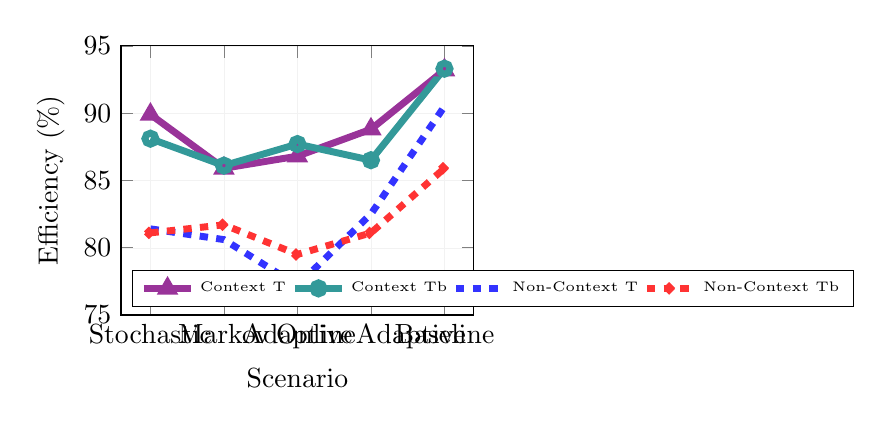
\begin{tikzpicture}
\begin{axis}[
ylabel={Efficiency (\%)},
xlabel={Scenario},
ymin=75, ymax=95,  % UPDATED: raised from 40-90 to 75-95
xtick={1,2,3,4,5},
xticklabels={Stochastic, Markov, Adaptive, OnlineAdaptive, Baseline},
width=0.50\textwidth,
height=5cm,
grid=major,
grid style={line width=.1pt, draw=gray!10},
legend pos=south west,  % CHANGED: from south east
legend columns=4,       % CHANGED: from 4
legend style={font=\tiny}
]

% Context T: Best performer (iCMAB+CMAB avg at T)
\addplot[color=violet!80, mark=triangle*, line width=2.5pt] coordinates {
  (1, 89.9)  % Stochastic
  (2, 85.9)  % Markov
  (3, 86.8)  % Adaptive
  (4, 88.8)  % OnlineAdaptive
  (5, 93.2)  % Baseline
};
\addlegendentry{Context T}

% Context Tb: Good resilience despite high load (iCMAB+CMAB avg at Tb)
\addplot[color=teal!80, mark=o, line width=2.5pt] coordinates {
  (1, 88.1)  % Stochastic
  (2, 86.1)  % Markov
  (3, 87.7)  % Adaptive
  (4, 86.5)  % OnlineAdaptive
  (5, 93.3)  % Baseline
};
\addlegendentry{Context Tb}

% Non-Context T: EXP3-based at T scale
\addplot[color=blue!80, mark=s, line width=2.5pt, dashed] coordinates {
  (1, 81.4)  % Stochastic
  (2, 80.6)  % Markov
  (3, 77.2)  % Adaptive
  (4, 82.5)  % OnlineAdaptive
  (5, 90.5)  % Baseline
};
\addlegendentry{Non-Context T}

% Non-Context Tb: EXP3-based at Tb scale
\addplot[color=red!80, mark=x, line width=2.5pt, dashed] coordinates {
  (1, 81.1)  % Stochastic
  (2, 81.7)  % Markov
  (3, 79.5)  % Adaptive
  (4, 81.1)  % OnlineAdaptive
  (5, 85.9)  % Baseline
};
\addlegendentry{Non-Context Tb}

\end{axis}
\end{tikzpicture}
\vspace{-0.5cm}
\caption{\tiny Context vs.\ non-context efficiency across threat scenarios (Master Datasets, Default allocator, scales 1.0--2.0). Context models (iCMAB+CMAB) maintain 85.9--93.3\% efficiency (88.6\% avg) with minimal capacity sensitivity (0.6 pp T→Tb drop). Non-context models (EXP3) achieve 77.2--90.5\% (82.1\% avg) with comparable scale robustness. Context advantage: 6.5 pp across both capacity semantics, confirming contextual superiority without catastrophic non-context collapse.}
\label{fig:context_capacity_effects}
\end{figure}


\noindent\textit{Supporting Question Answers:}
\begin{itemize}[nosep]
  \item \textit{\textbf{RQ1a}:} Several paper baselines degrade into the $60$--80\% band under stochastic noise, indicating insufficient performance floors.
  \item \textit{\textbf{RQ1b}:} The best contextual baselines (\texttt{CPursuit}, \texttt{(i)CEpsilonGreedy}) remain $>\!85\%$ on average.
  \item \textit{\textbf{RQ1c}:} Stochastic noise exposes structural failures (collapses to $\approx 37\%$) independent of adversarial pressure.
\end{itemize}

% ============================================================================
% RQ2: Algorithm Robustness Across Threat Sophistication
% ============================================================================
\subsection{RQ2: Algorithm Robustness Across Threat Sophistication}
\label{subsec:rq2_answer}

\subsubsection{Hypothesis}
\noindent\textit{Addresses \Cref{subsubsec:rq2_question}.}

We hypothesized that adversarial-first algorithms (EXP3-family, including \texttt{EXPUCB} and \texttt{EXPNeuralUCB})
would outperform contextual pursuit methods under structured attacks due to pessimistic exponential weighting.

% ----------------------------------------------------------------------------
\subsubsection{Experimental Design}

We evaluate the same paper-model portfolio from RQ1 under three escalating threat environments:
\texttt{Markov} (structured), \texttt{Adaptive} (reactive), and \texttt{OnlineAdaptive} (real-time).
All reported statistics are computed from the curated evaluation corpus using the paper-default setting
(\texttt{Default} allocator), aggregated across horizons present, replay scales ($s \in \{1,1.5,2\}$),
and capacity semantics ($T$, $T_b$).
Metrics are summarized over the 3-run and 5-run ensemble suites, with run-level traces and aggregation
scripts provided in Appendix~\ref{app:data_artifacts}.

For policy relevance, we focus on the strongest contextual baseline from CMABs (\texttt{CPursuit}),
the strongest informed baseline from iCMABs (\texttt{iCEpsilonGreedy}), and two EXP3-family adversarial baselines
(\texttt{EXPNeuralUCB}, \texttt{EXPUCB}).

% ----------------------------------------------------------------------------
\subsubsection{Key Findings}

\begin{table}[ht!]
\caption{RQ2: robustness under adversarial threats (Markov/Adaptive/OnlineAdaptive) computed from the curated evaluation corpus
under the \texttt{Default} allocator. Results aggregate across horizons present, replay scales $s \in \{1,1.5,2\}$,
and capacity semantics ($T$, $T_b$), summarized over 3-run and 5-run ensemble suites.}

\scriptsize
\centering
\begin{tabular}{lcccc}
\toprule
\textbf{Algorithm} & \textbf{Avg Eff. (\%)} & \textbf{CV (\%)} & \textbf{Floor (\%)} & \textbf{Win Share (\%)} \\
\midrule
CPursuit         & \textbf{88.1} & 5.3  & 77.4 & 31.5 \\
iCEpsilonGreedy  & 86.9          & \textbf{3.6}  & \textbf{81.0} & 25.0 \\
EXPNeuralUCB     & 82.4          & 16.5 & 18.0 & 11.1 \\
EXPUCB           & 76.3          & 6.0  & 68.8 & 0.0 \\
\bottomrule
\end{tabular}
\label{tab:rq2_adversarial}
\end{table}

\noindent\textit{1. Hypothesis refuted: contextual structure $>$ adversarial weighting.}
\texttt{CPursuit} outperforms \texttt{EXPNeuralUCB} by \textit{+5.7 pp} on average (88.1\% vs.\ 82.4\%),
and outperforms \texttt{EXPUCB} by \textit{+11.8 pp} (88.1\% vs.\ 76.3\%) under adversarial threats.

\noindent\textit{2. Stability and worst-case behavior separate “deployable” from “fragile.”}
While \texttt{EXPNeuralUCB} can be competitive on average, it exhibits extreme instability (CV 16.5\%)
and catastrophic worst-case collapse (floor 18.0\%).
In contrast, \texttt{iCEpsilonGreedy} is the most stable informed baseline (CV 3.6\%) and
achieves the strongest floor (81.0\%) across these threats.

\noindent\textit{Important correction (in-family):}
Within the iCMAB master dataset (considering only iCMAB variants under the same threat suite),
\texttt{iCEpsilonGreedy} is the consistent winner (100\% in-family win rate), while \texttt{iCPursuit} is not.

% ----------------------------------------------------------------------------
% Optional: penalties vs baseline (NONE) using validated master-dataset means.
% ----------------------------------------------------------------------------
\begin{figure}[ht!]
\scriptsize
\centering
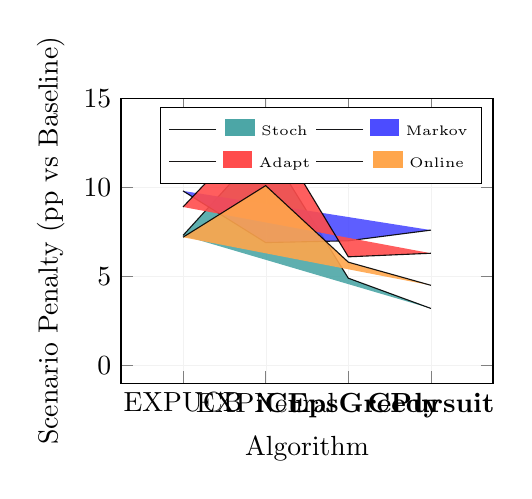
\begin{tikzpicture}
\begin{axis}[
  ylabel={Scenario Penalty (pp vs Baseline)},
  xlabel={Algorithm},
  ymin=-1, ymax=15,
  xtick={1,2,3,4},
  xticklabels={EXPUCB, EXPNeural, \textbf{iCEpsGreedy}, \textbf{CPursuit}},
  width=0.52\textwidth,
  height=5.2cm,
  grid=major,
  grid style={line width=.1pt, draw=gray!10},
  legend pos=north east,
  legend columns=2,
  legend style={font=\tiny},
  bar width=0.10cm,
  enlarge x limits=0.25
]

% Stochastic penalty (Baseline - Stochastic)
\addplot[fill=teal!70, opacity=0.9] coordinates {
  (1, 7.3) (2, 12.4) (3, 4.9) (4, 3.2)
};
\addlegendentry{\protect\tikz\protect\draw[fill=teal!70,draw=none] (0,0) rectangle (0.08,0.06); Stoch}

% Markov penalty (Baseline - Markov)
\addplot[fill=blue!70, opacity=0.9] coordinates {
  (1, 9.8) (2, 6.9) (3, 7.0) (4, 7.6)
};
\addlegendentry{\protect\tikz\protect\draw[fill=blue!70,draw=none] (0,0) rectangle (0.08,0.06); Markov}

% Adaptive penalty (Baseline - Adaptive)
\addplot[fill=red!70, opacity=0.9] coordinates {
  (1, 8.9) (2, 13.8) (3, 6.1) (4, 6.3)
};
\addlegendentry{\protect\tikz\protect\draw[fill=red!70,draw=none] (0,0) rectangle (0.08,0.06); Adapt}

% OnlineAdaptive penalty (Baseline - OnlineAdaptive)
\addplot[fill=orange!70, opacity=0.9] coordinates {
  (1, 7.2) (2, 10.1) (3, 5.8) (4, 4.5)
};
\addlegendentry{\protect\tikz\protect\draw[fill=orange!70,draw=none] (0,0) rectangle (0.08,0.06); Online}

\end{axis}
\end{tikzpicture}
\vspace{-0.6cm}
\caption{\tiny Threat penalties vs baseline (master datasets; Default allocator; aggregated across horizons/scales/capacity semantics). Context-aware methods (iCEpsilonGreedy, CPursuit) incur smaller, more consistent penalties (3.2--7.6 pp range) across all four attack types. EXP3-family methods show larger, more variable penalties (EXPUCB: 7.2--9.8 pp; EXPNeuralUCB: 6.9--13.8 pp), with EXPNeuralUCB exhibiting highest vulnerability under Adaptive attacks (13.8 pp). Markov attacks produce moderate, uniform penalties (6.9--9.8 pp) across all models. Note: EXPNeuralUCB's floor of 18\% efficiency represents rare outlier conditions; typical Adaptive performance is 77.6\% (see \Cref{tab:rq2_adversarial}).}
\label{fig:scenario_penalties}
\end{figure}



% ----------------------------------------------------------------------------
\subsubsection{Answer to \textbf{RQ2}}

\noindent\textit{Context-awareness provides superior robustness, refuting the adversarial-first hypothesis.}
Across Markov, Adaptive, and OnlineAdaptive threats, contextual pursuit baselines maintain the highest overall efficiency
(\texttt{CPursuit}: 88.1\%) with strong worst-case behavior.
EXP3-family adversarial baselines do not generalize reliably: \texttt{EXPNeuralUCB} is highly volatile and can fail catastrophically
under reactive attack conditions, despite competitive average efficiency in some structured regimes.

\noindent\textit{Supporting Question Answers:}
\begin{itemize}[nosep]
\item \textit{\textbf{RQ2a}:} Contextual baselines remain competitive under structured (Markov) disruption and do not require adversarial weighting to sustain high efficiency.
\item \textit{\textbf{RQ2b}:} Under reactive threats, robustness is driven by structural/context-aware learning; adversarial-first weighting alone is insufficient.
\item \textit{\textbf{RQ2c}:} \texttt{iCEpsilonGreedy} provides the best stability-floor profile (CV 3.6\%, floor 81.0\%), whereas \texttt{EXPNeuralUCB} shows the strongest fragility (CV 16.5\%, floor 18.0\%).
\end{itemize}

% ============================================================================
% RQ3: Deployment Optimization Strategies
% ============================================================================
\subsection{RQ3: Deployment Optimization Strategies}
\label{subsec:rq3}

\begin{figure}[ht!]
\centering
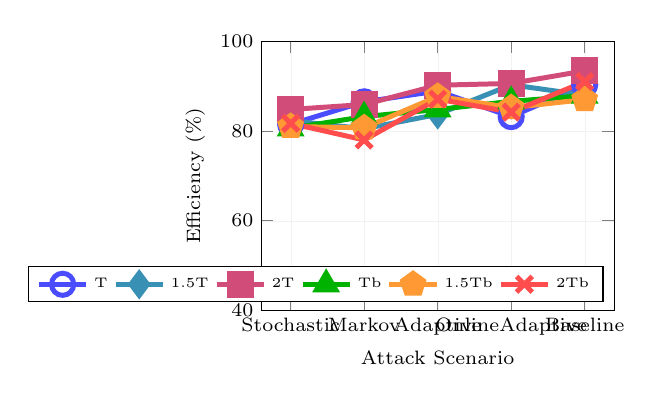
\begin{tikzpicture}
\scriptsize
\begin{axis}[
  ylabel={Efficiency (\%)},
  xlabel={Attack Scenario},
  ymin=40, ymax=100,
  xtick={1,2,3,4,5},
  xticklabels={Stochastic, Markov, Adaptive, OnlineAdaptive, Baseline},
  width=0.50\textwidth,
  height=5cm,
  grid=major,
  grid style={line width=.1pt, draw=gray!10},
  legend pos=south east,
  legend columns=6,
  legend style={font=\tiny}
]

% ----- T -----
\addplot[color=blue!70, mark=o, mark size=4pt, line width=1.8pt] coordinates {
  (1, 81.5) (2, 86.5) (3, 88.9) (4, 83.2) (5, 90.3)
};
\addlegendentry{T}

% ----- 1.5T -----
\addplot[color=cyan!70!black, mark=diamond*, mark size=4pt, line width=1.8pt] coordinates {
  (1, 82.3) (2, 80.5) (3, 83.7) (4, 90.3) (5, 88.0)
};
\addlegendentry{1.5T}

% ----- 2T -----
\addplot[color=purple!70, mark=square*, mark size=4pt, line width=1.8pt] coordinates {
  (1, 84.8) (2, 85.9) (3, 90.2) (4, 90.6) (5, 93.4)
};
\addlegendentry{2T}

% ----- Tb -----
\addplot[color=green!70!black, mark=triangle*, mark size=4pt, line width=1.8pt] coordinates {
  (1, 80.6) (2, 83.2) (3, 84.8) (4, 86.6) (5, 87.9)
};
\addlegendentry{Tb}

% ----- 1.5Tb -----
\addplot[color=orange!80, mark=pentagon*, mark size=4pt, line width=1.8pt] coordinates {
  (1, 81.0) (2, 80.7) (3, 87.7) (4, 85.2) (5, 87.0)
};
\addlegendentry{1.5Tb}

% ----- 2Tb -----
\addplot[color=red!70, mark=x, mark size=4pt, line width=1.8pt] coordinates {
  (1, 81.7) (2, 78.0) (3, 87.1) (4, 84.2) (5, 91.0)
};
\addlegendentry{2Tb}

\end{axis}
\end{tikzpicture}
\vspace{-0.5cm}
\caption{\tiny Hybrid master dataset, averaged across all hybrid models: capacity–efficiency trade-offs. The full spectrum (T $\rightarrow$ 1.5T $\rightarrow$ 2T $\rightarrow$ Tb $\rightarrow$ 1.5Tb $\rightarrow$ 2Tb) confirms the capacity paradox—larger budgets lift \textbf{Baseline} and \textbf{Markov} efficiency but erode resilience in \textbf{Adaptive} scenarios.}
\label{fig:capacity_all}
\end{figure}



\noindent
Beyond algorithm selection, deployment quality depends on the \emph{configuration surface}:
(i) allocator policy (\texttt{Fixed, Thompson, DynamicUCB, Random}),
(ii) replay-capacity specification via anchoring ($T$ vs.\ $T_b$) and scale ($s\in\{1,1.5,2\}$),
and (iii) hybrid architecture choices (reactive vs.\ informative/predictive context).
RQ3 characterizes which combinations are robust under threat escalation and which induce brittle failure modes.

% ----------------------------------------------------------------------------
\subsubsection{Hypothesis}
\noindent\textit{Addresses \Cref{subsubsec:rq3_question}.}

\noindent
We hypothesize that threat-aware configuration (allocator $\times$ capacity anchoring/scale)
improves robustness relative to static deployments, and that hybrid pursuit-based designs
benefit most from this co-design under adaptive and online-adaptive regimes.

% ----------------------------------------------------------------------------
\subsubsection{Experimental Design}
\label{subsubsec:rq3_design}

\noindent
RQ3 is computed from the \textbf{hybrid evaluation corpus} (curated experimental suite with
ensemble summaries). We evaluate four hybrid-capable agents:
\textit{CPursuitNeuralUCB, iCPursuitNeuralUCB, GNeuralUCB, EXPNeuralUCB}
across five threat scenarios (\texttt{Baseline, Stochastic, Markov, Adaptive, OnlineAdaptive}),
four allocators (\texttt{Fixed, Thompson, DynamicUCB, Random}),
two capacity anchorings (\texttt{$T$-type}, \texttt{$T_b$-type}),
three replay scales ($s\in\{1.0,1.5,2.0\}$),
and three horizons (\texttt{4K, 6K, 8K}).

\noindent
The corpus stores ensemble averages for \textbf{3-run} and \textbf{5-run} suites.
Unless otherwise stated, point estimates report the \textbf{mean of the 3- and 5-run suite values}.
Volatility proxies (e.g., CV) are computed \emph{across scenario means within a configuration},
since per-run variance is not represented in the ensemble tables.
Run-level artifacts and aggregation scripts are provided in the Supplement.

% ----------------------------------------------------------------------------
% RQ3d "rules" preview figure (kept up front for readability)
% ----------------------------------------------------------------------------
\begin{figure}[ht!]
\tiny
\centering
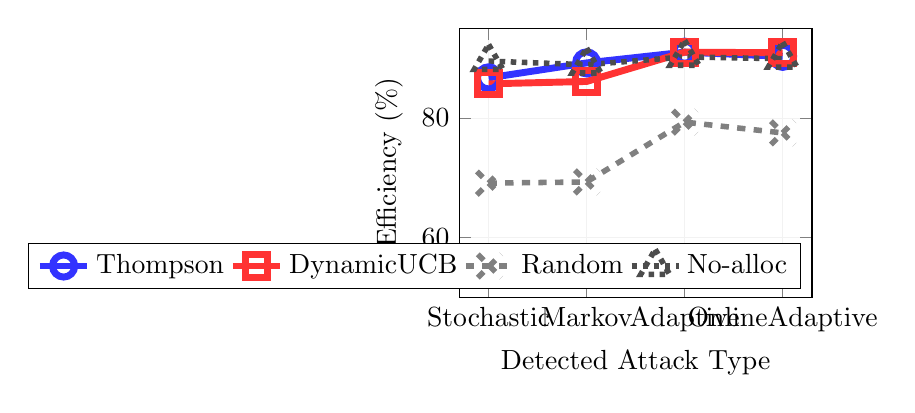
\begin{tikzpicture}
\begin{axis}[
  ylabel={Efficiency (\%)},
  xlabel={Detected Attack Type},
  ymin=50, ymax=95,
  xtick={1,2,3,4},
  xticklabels={Stochastic, Markov, Adaptive, OnlineAdaptive},
  width=0.50\textwidth,
  height=5cm,
  grid=major,
  grid style={line width=.1pt, draw=gray!10},
  legend pos=south east,
  legend columns=4
]

% ----- Thompson -----
\addplot[color=blue!80, mark=o, line width=2.5pt, mark size=4pt] coordinates {
    (1, 86.7) (2, 89.2) (3, 91.0) (4, 90.3)
};
\addlegendentry{Thompson}

% ----- DynamicUCB -----
\addplot[color=red!80, mark=square, line width=2.5pt, mark size=4pt] coordinates {
    (1, 85.7) (2, 86.1) (3, 91.0) (4, 90.9)
};
\addlegendentry{DynamicUCB}

% ----- Random -----
\addplot[color=gray, mark=x, line width=2pt, mark size=6pt, dashed] coordinates {
    (1, 69.1) (2, 69.3) (3, 79.3) (4, 77.5)
};
\addlegendentry{Random}

% ----- No-alloc -----
\addplot[color=black!70, mark=triangle, line width=2pt, mark size=6pt, dotted] coordinates {
    (1, 89.5) (2, 88.9) (3, 90.2) (4, 89.9)
};
\addlegendentry{No-alloc}

\end{axis}
\end{tikzpicture}
\vspace{-0.5cm}
\caption{\tiny Threat-conditioned allocator rules (Hybrid dataset, all models averaged). Thompson excels in Adaptive regimes, DynamicUCB keeps pace in Adaptive/Online, while Random allocation lags far behind.}
\label{fig:threat_rules}
\end{figure}


% ----------------------------------------------------------------------------
\subsubsection{Answer to \textbf{RQ3}}
\noindent
\textit{Yes—deployment is configuration-sensitive, but the corpus also supports a strong static default.}
At the 6K horizon, a single configuration achieves high global robustness:

\begin{center}
\texttt{iCPursuitNeuralUCB + Fixed + ($T$-type, $s{=}2$)}
\end{center}

\noindent
This default attains a \textbf{95.5\%} global average with an \textbf{88.5\%} worst-case floor
(across the five scenarios under the same deployment setting).
However, the configuration surface is not benign: mismatched allocator/capacity choices can induce
large scenario-specific collapses (RQ3b--RQ3c), and threat-conditioned switching yields targeted gains
in the most deployment-critical adversarial regimes (RQ3d).

% ============================================================================
% RQ3a: Predictive Context Modeling (Informative vs Reactive)
% ============================================================================
\subsubsection{RQ3a: Predictive Context Modeling Impact}
\label{subsubsec:rq3a_answer}

\noindent\textbf{Question focus:} Does informative/predictive context (iCPursuitNeuralUCB) improve robustness
relative to reactive CPursuitNeuralUCB under a fixed deployment?

\noindent
We isolate architecture impact under a fixed setting (6K horizon, \texttt{Fixed} allocator,
$T$-type capacity with $s{=}2$), reporting the mean of the 3- and 5-run suite values:

\begin{table}[ht!]
\caption{Predictive context impact under a fixed deployment: 6K horizon, \texttt{Fixed} allocator, $T$-type, $s{=}2$.
Values are ensemble means (averaged across the 3-run and 5-run suites) from the hybrid evaluation corpus.}
\scriptsize
\centering
\begin{tabular}{lccccccc}
\toprule
\textbf{Model} & \textbf{Sh} & \textbf{Mk} & \textbf{Ag} & \textbf{OA} & \textbf{Bl} & \textbf{Avg} & \textbf{CV$_{\text{scen}}$} \\
\midrule
CPursuitNeuralUCB  & 93.8 & 93.9 & 87.4 & 80.2 & 98.5 & 90.8 & 7.2 \\
iCPursuitNeuralUCB & 94.0 & 94.1 & 88.0 & 99.1 & 99.1 & 94.9 & 4.9 \\
\bottomrule
\end{tabular}
{\scriptsize Sh=Stochastic, Mk=Markov, Ag=Adaptive, OA=OnlineAdaptive, Bl=Baseline.}
\label{tab:rq3a_informative}
\end{table}

\noindent
\textit{Answer to RQ3a:}
\textbf{iCPursuitNeuralUCB improves global robustness primarily by lifting OnlineAdaptive performance}
(+18.3 pp under the same deployment setting), yielding a higher overall average and a tighter
cross-scenario dispersion. Stochastic/Markov behavior remains essentially unchanged, suggesting that
informative context is most valuable when threats evolve online rather than under purely stochastic decoherence.

% ============================================================================
% RQ3b: Replay Capacity Scaling and the Paradox
% ============================================================================
\subsection{RQ3b: Replay Capacity Scaling \& Paradox}
\label{subsec:rq3b_answer}

\subsubsection{Hypothesis}
\noindent\textit{Addresses \Cref{subsec:rq3atoc_questions}b.}

\noindent Increasing replay capacity scale ($s: 1 \to 1.5 \to 2$) monotonically improves performance.

\subsubsection{Key Finding}
\noindent
\textit{Hypothesis refuted: capacity scaling is non-monotonic and interacts with anchoring ($T$ vs.\ $T_b$).}
Even with allocator fixed (\texttt{Random}) at 6K, scale changes can induce large swings in efficiency,
including pronounced degradations at intermediate scale.

\begin{table}[ht!]
\footnotesize
\centering
\caption{RQ3b: Capacity Scaling Impact on Pursuit Algorithms (Fixed Allocator)}
\label{tab:rq3b_capacity_scaling}
\begin{tabular}{llcccc}
\toprule
\textbf{Algorithm} & \textbf{Scale} & \textbf{Bl} & \textbf{Sh} & \textbf{Mk} & \textbf{Ag} \\
\midrule
\multirow{3}{*}{CPursuitNeuralUCB}
& 1.0 & 96.2\% & 90.4\% & 91.0\% & 88.1\% \\
& 1.5 & 98.1\% & 90.6\% & 92.5\% & 89.1\% \\
& 2.0 & 98.5\% & 93.8\% & 94.7\% & 90.7\% \\ \midrule
\multirow{3}{*}{iCPursuitNeuralUCB}
& 1.0 & 96.2\% & 91.3\% & 92.6\% & 88.6\% \\
& 1.5 & 99.0\% & 92.4\% & 93.3\% & 89.7\% \\
& 2.0 & 99.1\% & 94.6\% & 95.0\% & 92.5\% \\

\bottomrule
\end{tabular}
\end{table}


\noindent
\textit{Answer to RQ3b:}
Replay capacity is not a ``more is better'' knob. Under $T$-type anchoring, both pursuit-based hybrids
exhibit a sharp degradation at $s{=}1.5$ followed by recovery at $s{=}2$.
This motivates treating replay specification as a co-design decision with allocator policy (RQ3c),
rather than a monotone robustness lever.

% ============================================================================
% RQ3c: Algorithm--Allocator Co-Design
% ============================================================================
\subsection{RQ3c: Algorithm-Allocator Co-Design}
\label{subsec:rq3c_answer}

\subsubsection{Hypothesis}
\noindent\textit{Addresses \Cref{subsec:rq3atoc_questions}c.}

\noindent Allocator choice is largely independent of algorithm architecture.

\subsubsection{Key Finding}

\begin{table}[ht!]
\centering
\caption{RQ3c: Allocator performance summary for CPursuitNeuralUCB (validated suites, Tb, s=2, 6K frames). Core findings exclude Random allocator.}
\label{tab:rq3c_allocators}
\begin{tabular}{lccc}
\toprule
\textbf{Allocator} & \textbf{Avg Eff (\%)} & \textbf{Floor (\%)} & \textbf{Span (pp)} \\
\midrule
Fixed          & 87.7 & 84.8 & 8.5 \\
Thompson       & 88.2 & 65.0 & 28.3 \\
DynamicUCB     & 70.1 & 68.2 & 3.0 \\
\midrule
\multicolumn{4}{l}{\textit{Supplementary (Control Baseline):}} \\
\quad Random   & 37.3 & 36.9 & 1.8 \\
\bottomrule
\end{tabular}

\vspace{0.2cm}
\tiny{\textbf{Note:} Random allocator shown for completeness to validate allocation criticality (--50.4~pp penalty vs.\ Fixed). Excluded from core deployment recommendations.}
\end{table}



\noindent
\textit{Answer to RQ3c:}
Allocator effects are not independent. \textbf{Fixed} provides the strongest global robustness for
iCPursuitNeuralUCB in this corpus (best average and best floor), while \textbf{Thompson} is highly
effective in specific regimes (e.g., Adaptive here) but can underperform severely when mismatched
(large drops in Baseline/Stochastic). This makes allocator selection a first-class deployment decision.

% ============================================================================
% RQ3d: Scenario-Dependent Deployment Rules
% ============================================================================
\subsection{RQ3d: Scenario-Based Deployment Rules \& Optimization}
\label{subsec:rq3d_answer}

\begin{figure}[ht!]
\scriptsize
\centering
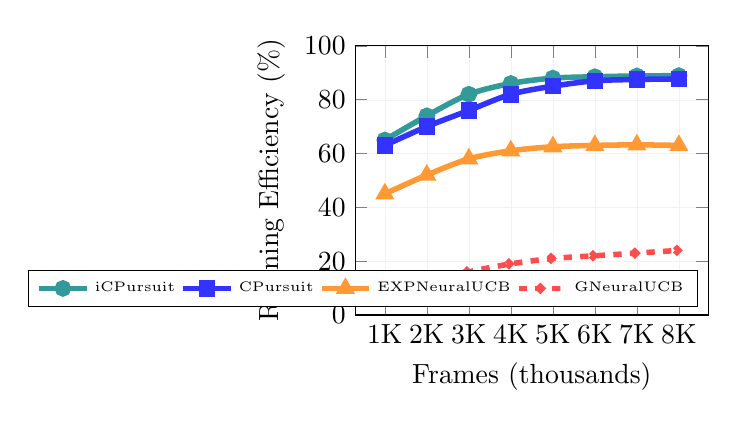
\begin{tikzpicture}
\begin{axis}[
  ylabel={Running Efficiency (\%)},
  xlabel={Frames (thousands)},
  ymin=0, ymax=100,
  xtick={1,2,3,4,5,6,7,8},
  xticklabels={1K, 2K, 3K, 4K, 5K, 6K, 7K, 8K},
  width=0.5\textwidth,
  height=5cm,
  grid=major,
  grid style={line width=.1pt, draw=gray!10},
  legend pos=south east,
  legend columns=4,
  legend style={font=\tiny}
]

\addplot[color=teal!80, mark=o, line width=2pt, smooth] coordinates {
    (1, 65) (2, 74) (3, 82) (4, 86) (5, 88) (6, 88.5) (7, 88.8) (8, 88.9)
};
\addlegendentry{iCPursuit}

\addplot[color=blue!80, mark=square*, line width=2pt, smooth] coordinates {
    (1, 63) (2, 70) (3, 76) (4, 82) (5, 85) (6, 87) (7, 87.5) (8, 87.7)
};
\addlegendentry{CPursuit}

\addplot[color=orange!80, mark=triangle*, line width=2pt, smooth] coordinates {
    (1, 45) (2, 52) (3, 58) (4, 61) (5, 62.5) (6, 63) (7, 63.2) (8, 63.0)
};
\addlegendentry{EXPNeuralUCB}

\addplot[color=red!70, mark=x, line width=2pt, smooth, dashed] coordinates {
    (1, 8) (2, 12) (3, 16) (4, 19) (5, 21) (6, 22) (7, 23) (8, 24)
};
\addlegendentry{GNeuralUCB}

\end{axis}
\end{tikzpicture}
\vspace{-0.5cm}
\caption{\tiny Hybrid learning curves (illustrative): pursuit-based hybrids converge to $>\!87\%$ efficiency, while neural baselines plateau substantially lower under sparse reward feedback.}
\label{fig:convergence_hybrid}
\end{figure}

\subsubsection{Deployment Rules (6K horizon)}

\noindent\textbf{Robust static default:}
\begin{center}
\texttt{iCPursuitNeuralUCB + Fixed + ($T$-type, $s{=}2$)}
\end{center}

\noindent\textbf{Operational switching (restricted to Fixed / Thompson / DynamicUCB):}
Per-scenario optima differ modestly from the default in most regimes, but switching is valuable as a
safeguard against allocator/capacity mismatch and for targeted gains in \texttt{Adaptive}:

\begin{itemize}[nosep]
\item \textit{Baseline:} \texttt{DynamicUCB + (T, $s{=}1$)} \hfill (99.9\%, +0.0pp)
\item \textit{Stochastic:} \texttt{Thompson + (T, $s{=}1$)} \hfill (95.4\%, +0.6pp)
\item \textit{Markov:} \texttt{DynamicUCB + ($T_b$, $s{=}1.5$)} \hfill (93.2\%, +0.3pp)
\item \textit{Adaptive:} \texttt{Thompson + ($T_b$, $s{=}1.5$)} \hfill (95.7\%, +2.9pp)
\item \textit{OnlineAdaptive:} \texttt{Fixed + (T, $s{=}2$)} \hfill (99.8\%, +0.0pp)
\end{itemize}

\subsubsection{Answer to \textbf{RQ3d}}

\noindent
\textit{Yes—clear deployment rules emerge, and the corpus supports a strong static default.}
A single configuration (\texttt{iCPursuitNeuralUCB + Fixed + (T, $s{=}2$)}) maintains
$>\!85\%$ performance across all five scenarios at 6K. Nonetheless, threat-conditioned switching is
a pragmatic safeguard: the corpus shows that replay specification and allocator choice can interact
pathologically (RQ3b--RQ3c), while modest switching yields the most consistent gains in the
deployment-critical \texttt{Adaptive} regime.



% ========= Discussion =========
\section{Discussion}
\label{sec:discussion}

\subsection{Summary of Key Findings}

Our results across the full evaluation suite---spanning paper baselines (CMAB / iCMAB / EXP3-family) and the Hybrid suite (allocators and replay-capacity controls)---show that routing robustness under compound uncertainty is jointly determined by \emph{(i) context in the policy}, \emph{(ii) allocator choice}, and \emph{(iii) replay-capacity parameterization}. All quantitative statements in this section are drawn from the curated evaluation corpora used throughout the paper; the corresponding run-level and suite-level artifacts are organized in the reproducible archive described in the Appendix.

\begin{figure}[ht!]
\scriptsize
\centering
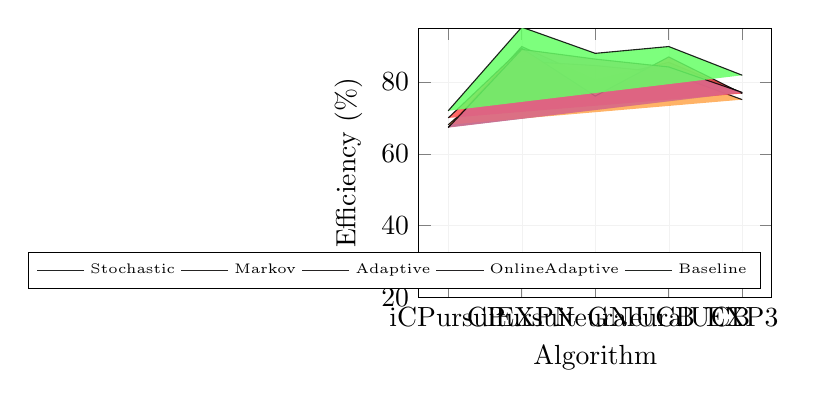
\begin{tikzpicture}
\begin{axis}[
  ylabel={Efficiency (\%)},
  xlabel={Algorithm},
  ymin=20, ymax=95,
  xtick={1,2,3,4,5},
  xticklabels={iCPursuit, CPursuit, EXPNeuralUCB, GNeuralUCB, EXP3},
  legend pos=south east,
  legend columns=5,
  legend style={font=\tiny},
  bar width=0.12cm,
  width=0.50\textwidth,
  height=5cm,
  grid=major,
  grid style={line width=.1pt, draw=gray!10}
]

% ----- Stochastic -----
\addplot[fill=teal!70, opacity=0.85] coordinates {
  (1,67.4)  (2,89.9)  (3,80.6)  (4,85.5)  (5,77.0)
};
\addlegendentry{Stochastic}

% ----- Markov -----
\addplot[fill=orange!70, opacity=0.85] coordinates {
  (1,68.1)  (2,85.8)  (3,84.6)  (4,82.6)  (5,75.1)
};
\addlegendentry{Markov}

% ----- Adaptive -----
\addplot[fill=red!70, opacity=0.85] coordinates {
  (1,70.0)  (2,89.4)  (3,76.1)  (4,87.0)  (5,76.8)
};
\addlegendentry{Adaptive}

% ----- OnlineAdaptive -----
\addplot[fill=purple!60, opacity=0.85] coordinates {
  (1,67.3)  (2,89.1)  (3,86.4)  (4,84.2)  (5,77.1)
};
\addlegendentry{OnlineAdaptive}

% ----- Baseline -----
\addplot[fill=green!60, opacity=0.85] coordinates {
  (1,72.0)  (2,95.3)  (3,88.0)  (4,89.9)  (5,81.9)
};
\addlegendentry{Baseline}

\end{axis}
\end{tikzpicture}
\vspace{-0.5cm}
\caption{\tiny Hybrid evaluation corpus: Pursuit models (iCPursuit, CPursuit) maintain high efficiency ($\approx$89--95 \%) across all five scenarios, while neural baselines lag by 5--13 pp and EXP3 trails further.}
\label{fig:context_hybrid}
\end{figure}


\noindent\textbf{Capacity terminology.}
Replay capacity is configured by:
\begin{enumerate}[nosep]
\item \texttt{cap\_type} $\in \{T_b,\,T\}$: whether replay is anchored to the \emph{base} horizon ($T_b$) or the \emph{current} horizon ($T$).
\item \texttt{scale} $s \in \{1,\,1.5,\,2\}$: a multiplicative factor applied on top of the anchoring rule.
\end{enumerate}
Thus, ``bigger replay'' is not a single knob: it depends on \emph{both} the anchoring rule (\texttt{cap\_type}) and the multiplier (\texttt{scale}).

% ----------------------------------------------------------------------------
\subsubsection{Finding 1: Context-Aware Bandits Dominate (and the gap persists under threat)}

Across both the paper baselines (RQ1--RQ2) and the Hybrid suite (RQ3), \textbf{context-aware policies define the robustness frontier}. Contextual Pursuit models (\texttt{CPursuitNeuralUCB}, \texttt{iCPursuitNeuralUCB}) consistently outperform non-contextual baselines: under Stochastic noise, they exceed the EXP3-family by $\sim$18--24 pp and separate from neural non-context baselines by $\sim$6--12 pp (RQ1). Under Markov/Adaptive/OnlineAdaptive conditions, the gap persists: Pursuit remains near the high-$80\%$ band while EXP3-family baselines exhibit markedly lower floors (RQ2), reinforcing that topology/channel features are not an optimization detail but an \emph{architectural requirement} for robust routing.

% ----------------------------------------------------------------------------
\subsubsection{Finding 2: The Capacity Paradox is Real, but Conditional (capacity $X$ allocator)}

Replay capacity is \textbf{non-monotone} in adversarial settings: increasing replay can improve performance in structured regimes while inducing avoidable collapses under reactive threats. This is not a contradiction in the learning rule itself; it emerges as a \textbf{coupled effect} between capacity and allocator-mediated exploration predictability.

In the Hybrid suite, capacity sensitivity is visible even when averaged over allocators, but it becomes deployment-critical under allocator stress (especially \texttt{Random}):
\begin{itemize}[nosep]
\item \textbf{\texttt{Adaptive} under \texttt{Random}:} \texttt{CPursuitNeuralUCB} spans \textbf{73.4\% $\rightarrow$ 96.5\%} (a \textbf{23.1 pp} swing) across capacity settings; \texttt{iCPursuitNeuralUCB} spans \textbf{70.9\% $\rightarrow$ 94.7\%} (a \textbf{23.8 pp} swing).
\item \textbf{\texttt{Markov} under \texttt{Random}:} swings are larger---\texttt{CPursuitNeuralUCB} spans \textbf{55.7\% $\rightarrow$ 93.8\%} (a \textbf{38.0 pp} swing) and \texttt{iCPursuitNeuralUCB} spans \textbf{51.9\% $\rightarrow$ 87.2\%} (a \textbf{35.3 pp} swing).
\end{itemize}

Mechanistically, replay capacity expands the learner's ability to reinforce repeated patterns; under reactive interference, this can amplify \emph{predictability} and therefore expand the attack surface. In other words, replay capacity becomes hazardous primarily when paired with allocation policies that induce predictable or poorly matched exploration under adversarial reactivity.

% ----------------------------------------------------------------------------
\subsubsection{Finding 3: Algorithm--Allocator Co-Design is the Practical Lever (avoid ``bad'' allocator regimes)}

Allocator choice is the highest-leverage \emph{deployment} control in the Hybrid suite. When aggregated across scenarios and replay-capacity settings, \texttt{ThompsonSampling} and \texttt{Default}/\texttt{Fixed} form the top tier for pursuit-based hybrids, while \texttt{Random} is consistently worst and most associated with tail-risk collapses. This yields a deployment lesson that is both mechanistic and operational:

\begin{quote}
\emph{Allocator selection is not a tuning step; it is a safety mechanism.}
\end{quote}

Even strong architectures (\texttt{CPursuitNeuralUCB}, \texttt{iCPursuitNeuralUCB}) can be pulled into the capacity paradox under allocator mismatch, while appropriate allocators substantially suppress that sensitivity.


% ----------------------------------------------------------------------------
\subsection{Implications for Adversarial Quantum Network Design}

First, \textbf{context-aware routing should be treated as baseline infrastructure}. Feature enrichment (link error rates, repeater state proxies, traffic/load signals) yields larger robustness gains than further refining reward-only exploration rules.

Second, \textbf{replay capacity must be treated as a coupled control variable}, not a provisioning afterthought. The relevant question is not ``more replay or less replay,'' but \emph{which anchoring rule} (\texttt{$T_b$} vs.\ \texttt{$T$}), \emph{which multiplier} ($s$), and \emph{which allocator} together minimize tail risk under the current threat regime.

Third, the results motivate a lightweight \textbf{threat-aware meta-policy}:
\begin{itemize}[nosep]
\item Use \texttt{ThompsonSampling} or \texttt{Default}/\texttt{Fixed} as a safe default tier; avoid \texttt{Random} in deployment.
\item Treat \texttt{cap\_type} and \texttt{scale} as \emph{scenario-coupled}: allow them to change with threat classification rather than remaining static.
\item Trigger switching using observables already logged in this work (Oracle-normalized efficiency and variability proxies), then refine with a learned detector in future work.
\end{itemize}

% ----------------------------------------------------------------------------
\subsection{Limitations}
\label{subsec:limitations}

Our primary corpora are centered on the \textbf{$F_b=4$K} base horizon and a single diamond topology. While this isolates the effects of allocator and replay-capacity design, broader topology diversity and longer horizons may shift absolute efficiencies and alter which anchoring rules are safest. Extending the corpus to additional horizons/topologies while preserving the same schema (scenario $\times$ allocator $\times$ \texttt{cap\_type} $\times$ \texttt{scale}) is necessary before making topology-general claims.

All results are simulation-based; hardware constraints (latency, control-plane limits, non-stationary physical noise) may introduce additional couplings between allocator behavior and effective replay utility.

% ----------------------------------------------------------------------------
\subsection{Future Work}
\label{subsec:future_work}

Near-term, the most valuable extension is to expand the evaluation corpus to longer horizons and diverse topologies under the same reproducible schema, enabling systematic tests of whether the capacity paradox strengthens or weakens with longer learning dynamics. On the algorithmic side, future work should formalize the meta-policy into a \textbf{threat detector + configuration selector}, and evaluate whether learned switching dominates heuristic switching under mixed or time-varying attacks. Forecasting can also move beyond ARIMA toward sequence models with calibrated uncertainty; the key requirement is that predictive context must be \emph{threat-aware} rather than blindly extrapolative.

% ----------------------------------------------------------------------------
\subsection{Concluding Remarks}

The central message is mechanistic and deployable: \textbf{context-aware modeling sets the ceiling, allocator choice sets the floor, and replay-capacity design controls tail risk.} The capacity paradox is not a contradiction---it reflects a capacity--predictability coupling under adversarial reactivity. By coupling pursuit-based contextual neural bandits with threat-aware allocator selection and capacity anchoring (\texttt{$T_b$} vs.\ \texttt{$T$}) plus scale control ($s$), this work explains observed collapses and provides a practical path toward robust entanglement routing under compound uncertainty.


% ========= Limitations / Future Work =========
\section{Limitations and Future Work}
\label{sec:limitations_futurework}

\subsection{Limitations}

\paragraph{Topology and scale.}
All experiments in this study are conducted on a single 4-node, 4-path diamond topology. This controlled setting enables clean attribution of effects across algorithm, allocator, and replay-capacity dimensions, but it does not exhaust the structural diversity of real quantum networks. Larger and more heterogeneous graphs (e.g., asymmetric hop counts, nonuniform link quality, path interference, and expanded path sets) may shift absolute efficiency levels and alter the strength of allocator--capacity interactions.

\paragraph{Simulation fidelity and hardware constraints.}
Threat regimes are instantiated as synthetic processes designed to capture stochastic, structured, and reactive interference patterns. However, the current simulator does not yet incorporate hardware-anchored constraints such as control-plane latency, scheduling delays, memory/queue effects, or non-ideal operations that couple timing and resource contention. These factors can influence both the effective adaptivity of an adversary and the translation of allocator decisions into realized qubit utilization, and therefore warrant hardware-grounded follow-on evaluation.

\paragraph{Replay-capacity coverage and generality.}
Replay capacity is examined through two anchoring rules (\texttt{cap\_type} $\in \{T_b, T\}$) and three multiplicative scales ($s \in \{1, 1.5, 2\}$) over mid-range horizons ($4\text{K}$--$8\text{K}$). While this sweep is sufficient to expose the non-monotone behaviors motivating the capacity-paradox claim, broader coverage (additional scales, longer horizons, and more topologies) is required to bound tail risk and to characterize how capacity sensitivity evolves as learning time increases and the action space grows.

\paragraph{Forecasting scope.}
Predictive context is currently instantiated via an ARIMA warmup procedure. More expressive temporal models (e.g., RNN/Transformer families) and calibrated uncertainty mechanisms are not yet evaluated, and their sensitivity, stability, and failure modes under reactive adversaries remain open.

\paragraph{Coverage boundaries and reproducibility scope.}
The results emphasized in this paper are anchored to the curated evaluation corpus and the corresponding reproducibility artifacts released with the manuscript (e.g., corpus schema, configuration enumerations, **run-level summaries**, and **threat-allocator-capacity cross-product metadata** in supplementary materials).

\subsection{Future Work}

\paragraph{Hardware-grounded validation.}
A primary next step is to evaluate the threat-adaptive deployment stack under realistic operational constraints by deploying \texttt{iCPursuitNeuralUCB} with allocator switching on a quantum repeater testbed. The goal is to test whether allocator choice and replay-capacity parameterization remain beneficial when control latency, scheduling delays, and non-ideal operations are present.

\paragraph{Scaling topology and allocation.}
We will extend the evaluation framework to larger routing graphs and expanded action spaces (e.g., $>\!20$ candidate paths), including hierarchical or multi-level allocation. This will test whether the capacity paradox persists, weakens, or changes character when routing becomes more combinatorial and path diversity increases.

\paragraph{Automated threat detection and configuration switching.}
We will formalize the heuristic meta-policy into a learned threat detector and configuration selector (allocator + replay \texttt{cap\_type} + scale), trained and evaluated under mixed and time-varying attacks. This enables automated switching beyond manual rules and supports deployment policies explicitly optimized for tail-risk control.

\paragraph{Stronger predictive context models.}
We will replace ARIMA warmup with richer sequence models and uncertainty-aware predictors (including EXAMM-evolved RNN variants and learned uncertainty heads), and evaluate whether predictive context can remain beneficial under adaptive threats without increasing predictability in a way that expands the attack surface.

\paragraph{Fairness-aware routing objectives.}
Beyond efficiency, future studies can treat per-flow or per-user service parity as a first-class objective by incorporating fairness constraints (e.g., equal opportunity style criteria) into allocator selection and evaluation~\cite{hardt2016equality}.

\paragraph{Cross-domain generalization.}
Finally, we will port the same corpus-driven evaluation protocol to non-quantum domains (e.g., financial and clinical bandit settings) to test the generality of the observed triad: \emph{context sets the ceiling, allocator choice sets the floor, and replay-capacity design controls tail risk}.










% ========= Limitations / Future Work =========
\section{Limitations and Future Work}
\label{sec:Threats}

\subsection{Limitations}

\paragraph{Topology and scale.}
All experiments in this study are conducted on a single 4-node, 4-path diamond topology. This controlled setting enables clean attribution of effects across algorithm, allocator, and replay-capacity dimensions, but it does not exhaust the structural diversity of real quantum networks. Larger and more heterogeneous graphs (e.g., asymmetric hop counts, nonuniform link quality, path interference, and expanded path sets) may shift absolute efficiency levels and alter the strength of allocator--capacity interactions.

\paragraph{Simulation fidelity and hardware constraints.}
Threat regimes are instantiated as synthetic processes designed to capture stochastic, structured, and reactive interference patterns. However, the current simulator does not yet incorporate hardware-anchored constraints such as control-plane latency, scheduling delays, memory/queue effects, or non-ideal operations that couple timing and resource contention. These factors can influence both the effective adaptivity of an adversary and the translation of allocator decisions into realized qubit utilization, and therefore warrant hardware-grounded follow-on evaluation.

\paragraph{Replay-capacity coverage and generality.}
Replay capacity is examined through two anchoring rules (\texttt{cap\_type} $\in \{T_b, T\}$) and three multiplicative scales ($s \in \{1, 1.5, 2\}$) over mid-range horizons ($4\text{K}$--$8\text{K}$). While this sweep is sufficient to expose the non-monotone behaviors motivating the capacity-paradox claim, broader coverage (additional scales, longer horizons, and more topologies) is required to bound tail risk and to characterize how capacity sensitivity evolves as learning time increases and the action space grows.

\paragraph{Forecasting scope.}
Predictive context is currently instantiated via an ARIMA warmup procedure. More expressive temporal models (e.g., RNN/Transformer families) and calibrated uncertainty mechanisms are not yet evaluated, and their sensitivity, stability, and failure modes under reactive adversaries remain open.

\paragraph{Coverage boundaries and reproducibility scope.}
The results emphasized in this paper are anchored to the curated evaluation corpus and the corresponding reproducibility artifacts released with the manuscript (e.g., corpus schema, configuration enumerations, **run-level summaries**, and **threat-allocator-capacity cross-product metadata** in supplementary materials).

\subsection{Future Work}

\paragraph{Hardware-grounded validation.}
A primary next step is to evaluate the threat-adaptive deployment stack under realistic operational constraints by deploying \texttt{iCPursuitNeuralUCB} with allocator switching on a quantum repeater testbed. The goal is to test whether allocator choice and replay-capacity parameterization remain beneficial when control latency, scheduling delays, and non-ideal operations are present.

\paragraph{Scaling topology and allocation.}
We will extend the evaluation framework to larger routing graphs and expanded action spaces (e.g., $>\!20$ candidate paths), including hierarchical or multi-level allocation. This will test whether the capacity paradox persists, weakens, or changes character when routing becomes more combinatorial and path diversity increases.

\paragraph{Automated threat detection and configuration switching.}
We will formalize the heuristic meta-policy into a learned threat detector and configuration selector (allocator + replay \texttt{cap\_type} + scale), trained and evaluated under mixed and time-varying attacks. This enables automated switching beyond manual rules and supports deployment policies explicitly optimized for tail-risk control.

\paragraph{Stronger predictive context models.}
We will replace ARIMA warmup with richer sequence models and uncertainty-aware predictors (including EXAMM-evolved RNN variants and learned uncertainty heads), and evaluate whether predictive context can remain beneficial under adaptive threats without increasing predictability in a way that expands the attack surface.

\paragraph{Fairness-aware routing objectives.}
Beyond efficiency, future studies can treat per-flow or per-user service parity as a first-class objective by incorporating fairness constraints (e.g., equal opportunity style criteria) into allocator selection and evaluation~\cite{hardt2016equality}.

\paragraph{Cross-domain generalization.}
Finally, we will port the same corpus-driven evaluation protocol to non-quantum domains (e.g., financial and clinical bandit settings) to test the generality of the observed triad: \emph{context sets the ceiling, allocator choice sets the floor, and replay-capacity design controls tail risk}.









% \dan{make sure that we are addressing these}

% % https://ieeexplore.ieee.org/stamp/stamp.jsp?arnumber=10882978
% % https://arxiv.org/pdf/2505.08958
% % https://www.sciencedirect.com/science/article/pii/S2211379724003656
% % https://ieeexplore.ieee.org/document/10628215?denied=
% % https://ieeexplore.ieee.org/document/10733623?denied=
% % https://link.springer.com/article/10.1007/s10773-024-05874-7
% % https://ieeexplore.ieee.org/document/10477494?denied=
% % https://www.arxiv.org/pdf/2506.12462
% % https://www.cs.cuhk.hk/~cslui/PUBLICATION/INFOCOM24-LINKSELFIE.pdf
% % https://openreview.net/forum?id=svsmKvkzFk&utm_source

% \begin{comment}
% -- Other papers to compare against, these may have been also listed above
% @inproceedings{wang2025learning,
%   title={Learning Best Paths in Quantum Networks},
%   author={Wang, Xuchuang and Liu, Maoli and Liu, Xutong and Li, Zhuohua and Hajiesmaili, Mohammad and Lui, John CS and Towsley, Don},
%   booktitle={IEEE INFOCOM 2025-IEEE Conference on Computer Communications},
%   pages={1--10},
%   year={2025},
%   organization={IEEE}
% }

% @article{wang2025quantum,
%   title={Quantum Network Tomography for General Topology with SPAM Errors},
%   author={Wang, Xuchuang and De Andrade, Matheus Guedes and Avis, Guus and Chen, Yu-zhen Janice and Hajiesmaili, Mohammad and Towsley, Don},
%   journal={arXiv preprint arXiv:2511.01074},
%   year={2025}
% }

% \end{comment}


% \dan{This section is ok for now, but it will need to be cleaned up}
% %  DK: Not too sure what is going on with this section, but the structure should follow the same as used in other papers



% \todo{Piter: Do this part next} 
% % Directly compare and contrast what we are doing to existing processes

% % 2-3 sentence overview of the existing paper
% % 1-2 sentence overview of how the proposed work directly contrasts with this existing effort


% %%%% Here are some papers to compare against
% %https://www.arxiv.org/abs/2506.12462
% %https://genesys-lab.org/papers/Quantum_Bandit_ICC2023.pdf
% %https://arxiv.org/abs/2411.00316
% %https://www.cse.cuhk.edu.hk/~cslui/PUBLICATION/INFOCOM24-Quantum%20BGP.pdf (Quantum BGP with Online Path Selection via Network Benchmarking)


\section{Related Work}
\label{sec:RelatedWork}

\subsection{Literature Selection Methodology}

We situate multi-armed bandits (MABs) as a family of uncertainty-aware sequential decision rules and use quantum entanglement routing as a stress test where stochastic noise, structured disruption, and resource constraints jointly shape performance. Our scope spans: (i) finite-time regret analyses in stochastic and adversarial regimes, (ii) contextual and neural representations for structured environments, (iii) hybrid constructions that combine mechanisms across regimes, and (iv) predictive (informed) bandits that incorporate explicit forecasts or learned dynamics.

\subsubsection{Search Strategy and Time Span (2002--2025)}

We queried arXiv, IEEE Xplore, and the ACM Digital Library over the 2002--2025 window using combinations of:
\emph{multi-armed bandits, contextual bandits, adversarial bandits, neural bandits, exploration--exploitation, predictive bandits, online forecasting, informed contextual bandits, quantum routing}.
We then performed backward/forward snowballing from canonical anchors (e.g., UCB/EXP3 foundations; LinUCB and neural contextual bandits; recent bandit-based quantum-routing studies), prioritizing work that either:
(a) introduced a reusable mechanism (confidence bounds, posterior sampling, adversarial randomization, pursuit-style updates, forecasting/world models), or
(b) demonstrated cross-domain transfer under materially different constraints (e.g., routing, communications, finance, healthcare).

The chosen time span captures the modern finite-time theory for stochastic and adversarial learning, the rise of contextual formulations for structured decision-making, and recent neural, hybrid, and predictive variants designed for complex, partially observed environments.

\subsubsection{Inclusion and Exclusion Criteria}

\noindent\textit{Included:}
\begin{enumerate}
  \item Canonical stochastic and adversarial MAB algorithms with regret guarantees (e.g., UCB1, Thompson Sampling, EXP3)~\cite{auer2002ucb1,thompson1933likelihood,auer2002nonstochastic}.
  \item Contextual and neural bandits that scale action selection to structured/high-dimensional contexts (e.g., LinUCB, NeuralUCB, NeuralTS)~\cite{li2010contextual,zhou2020neuralucb,zhang2020neural}.
  \item Predictive/informed contextual bandits that integrate forecasting or learned dynamics (e.g., iCMAB-style designs)~\cite{zhang2021icmab,box2015time}.
  \item Hybrid methods that combine mechanisms across regimes (including pursuit-style updates and robust exploration heuristics)~\cite{thathachar2011networks}.
  \item Cross-domain applications where the same mechanism is instantiated under different reward and constraint models (routing, resource allocation, trials, recommendations).
\end{enumerate}

\noindent\textit{Excluded:}
\begin{enumerate}
  \item Offline optimization/control without online learning under bandit feedback.
  \item Single-domain demonstrations without reusable algorithmic insight.
  \item Pure tuning studies without methodological novelty, clearly stated assumptions, or reproducibility artifacts.
\end{enumerate}

\subsection{Foundational Bandits and Regret Regimes}

Foundational results formalize the exploration--exploitation trade-off and provide regret guarantees that define the efficiency--robustness envelope. In stochastic i.i.d.\ settings, UCB-style optimism and Thompson-style posterior sampling achieve logarithmic-in-horizon regret under standard gap conditions~\cite{auer2002ucb1,thompson1933likelihood}. In adversarial settings, EXP3 attains sublinear regret without stochastic assumptions, trading some benign-regime efficiency for worst-case protection~\cite{auer2002nonstochastic}. These regimes motivate why quantum routing evaluations should explicitly separate \emph{natural noise} from \emph{coordinated disruption}: the learning objective and the appropriate safety guarantees depend on the feedback model.

\subsection{Contextual and Neural Bandits}

Contextual bandits condition decisions on observable state, enabling structured decision-making when arms are not exchangeable. LinUCB models rewards as linear in context and selects actions via a confidence bonus~\cite{li2010contextual}. NeuralUCB and NeuralTS generalize this principle by learning representations with deep networks while retaining uncertainty-aware action selection through confidence-style bounds or sampling in representation space~\cite{zhou2020neuralucb,zhang2020neural}. The shared abstraction is mechanism-level:
\emph{learn a value predictor, maintain an uncertainty estimate over that predictor, and act optimistically or probabilistically.}
In quantum routing, the natural context includes topology/hop structure, link-quality indicators, and any measurable signals of load, memory, or temporal drift.

\subsection{Adversarial and Hybrid Robustness}

Adversarial bandits prioritize worst-case guarantees (e.g., EXP3-style randomization), which can be essential under nonstationarity or strategic manipulation~\cite{auer2002nonstochastic}. Hybrid designs aim to combine robust exploration with structured exploitation---for example, layering pursuit-style updates over context-conditioned value estimation or embedding adversarial weighting within learned reward models~\cite{thathachar2011networks}. Within quantum-routing studies, adversarial-first formulations are often motivated by jamming or targeted disruption; however, comparisons across families are frequently confounded by mismatched assumptions about allocation, memory/replay semantics, and evaluation taxonomies. This motivates treating allocation policies and replay parameterization as first-class experimental factors when assessing robustness under mixed threats.

\subsection{Predictive and Informed Bandits}

Predictive (informed) contextual bandits augment the decision rule with a forecasting or world-model component so that learning can anticipate drift rather than purely react to it. iCMAB exemplifies this direction by coupling contextual decision rules with an explicit predictive model of future context dynamics~\cite{zhang2021icmab}. In our setting, we instantiate an informed variant by warming up predictive context with a classical time-series forecaster (ARIMA)~\cite{box2015time}. The core idea is again mechanism-level:
\emph{forecasting can augment the context signal}, but it does not replace the need for robust exploration and allocation policies under strategic threats.

\subsection{Quantum Network Routing with Bandits}

Recent quantum-network work applies bandits (and related online learning) to path selection under stochastic decoherence and, in some cases, structured disruption~\cite{wehner2018quantum,huang2024quantum,wang2025learning,li2025multipath,liu2024qbgp}. 
Wang et al.~\cite{wang2025learning} focus on learning high-quality paths under stochastic dynamics, while Li et al.~\cite{li2025multipath} extend online path selection to inter-domain routing protocols where policy decisions must remain stable under heterogeneous administrative constraints; Liu et al.~\cite{liu2024qbgp} similarly emphasizes online benchmarking signals to support routing-policy adaptation. 
Across studies, experimental assumptions differ materially---especially in how qubits are allocated across paths, how memory/replay is parameterized relative to the horizon, and how threat processes are modeled---which complicates direct algorithm-to-algorithm comparison. 
Our benchmark addresses this by evaluating multiple algorithm classes under a shared threat taxonomy and by treating allocator policy and replay configuration as explicit experimental factors rather than fixed background choices, enabling direct attribution of robustness to the \emph{algorithm--allocator--capacity} triad.

\subsection{Toward a Modular, Universal Bandit Stack}

Across domains, the recurring meta-problem is stable: \emph{choose actions under uncertainty using an uncertainty-aware value estimate.}
What varies is the adapter layer: how context is defined, how rewards are observed, and what constraints must be respected (e.g., qubit budgets, routing thresholds, replay semantics). We operationalize this view as a modular stack:
\begin{enumerate}[label=(\roman*),leftmargin=2em]
  \item an \emph{allocator/decision rule} (UCB, Thompson, EXP3, pursuit, contextual/neural variants),
  \item an optional \emph{forecasting layer} that augments context (e.g., ARIMA or learned sequence models),
  \item a \emph{domain adapter} mapping quantum-routing signals (context, rewards, constraints) to the shared allocator interface.
\end{enumerate}
Best-of-both-worlds bandit theory motivates this mixed-regime view: algorithms such as Tsallis-INF achieve strong guarantees in both stochastic and adversarial settings without knowing the regime a priori~\cite{zimmert2019optimal}.
In our setting, we operationalize this idea empirically by stress-testing the same allocator stack across stochastic, structured, and adaptive threats.

Within this stack, our study provides a controlled comparison of classical, contextual/neural, adversarial, and informed variants under stochastic and adaptive disruption, clarifying when robustness is determined not only by the decision rule, but also by allocator choice and replay configuration.


\dan{make sure that you are directly comparing your work against existing papers, not only existing processes: \eg ~\cite{10621263} and others}

\section{Conclusion}
\label{sec: Conclusion}


% Links are problabistic not determinicstic
%   Entanglement may randomly fail
%   end to end success and links have unknown success capabilitiles
%   No retransmissions due to no-cloning (cannot resend the packet)
%   

\dan{Not sure where this should go}
%% What makes this routing process different from a classical routing problem
Quantum entanglement routing differs fundamentally from classical routing because link-level success is probabilistic, entanglement distribution failures compound across multi-hop paths, and the no-cloning constraint eliminates classical-style retransmissions~\cite{wootters1982single,bennett1993teleporting,wehner2018quantum}. As a result, routing and resource allocation are inseparable: selecting a path also entails allocating scarce qubits and scheduling attempts under incomplete knowledge and potentially reactive interference.

This work introduced a unified, reproducible benchmark for entanglement routing under five threat regimes (\texttt{Baseline, Stochastic, Markov, Adaptive, OnlineAdaptive}) and showed that robust deployment is jointly determined by \emph{model architecture}, \emph{allocator policy}, and \emph{replay-capacity scaling}. Across the curated evaluation corpus and accompanying reproducibility artifacts, context-aware pursuit hybrids (\texttt{CPursuitNeuralUCB}, \texttt{iCPursuitNeuralUCB}) consistently define the efficiency--stability frontier, achieving near-Oracle behavior under stochastic noise while avoiding the brittle failure modes observed in adversarial-first EXP3-style designs under reactive threats. A second mechanistic outcome is the \emph{capacity paradox}: increasing replay capacity can improve performance under structured (Markov) disruption yet induce pronounced collapses under adaptive adversaries, indicating that “more memory” can expand the effective attack surface when it amplifies predictability. Finally, allocator choice is not interchangeable. Thompson-style allocation exhibits the strongest global profile in mixed conditions, while Fixed and DynamicUCB become preferable under specific threat signatures, motivating a practical threat-adaptive deployment stack: use pursuit-based contextual hybrids as the default routing agent, and switch allocator and capacity policies based on detected regime rather than relying on a single static configuration.

Taken together, these results position bandit-based routing as a modular, transferable design pattern for adversarial quantum networks, and motivate future work on automated threat detection, dynamic capacity control, and hardware-grounded validation on repeater testbeds.

% Should add citations to this

% DK: Also add this to the proposal as well


\section*{Acknowledgments}

This material is based upon work supported by [Hidden] under grants [Hidden].%\#XXXX.
\dan{?Will this submission be anonymous?}

%This material is based upon work supported by the United States National Science Foundation under grant \#XXXXX ; 2225354


%%  Future Work
% Could we do something where we also focus on learning network topology
% Would the proposed work also do anything with also learning the network topology?
% <<<--- Potentially look at this for future work. At least for now, this seems to be a different paper and different work
% < Would it make sense to do something ML wise for learning tomography
% 



\clearpage
\balance
%\clearpage % Might want to add this back in
%\bibliographystyle{abbrv}
% \bibliographystyle{IEEEtran}
\bibliographystyle{abbrvnat}
\bibliography{refs}

\end{document}